\documentclass[review,12pt]{elsarticle}
\biboptions{authoryear}
\usepackage{amssymb,amsmath,amsthm}
\usepackage{booktabs}
\usepackage{multirow}
\usepackage{enumitem}
\usepackage{graphicx}
\usepackage[colorlinks=true,linkcolor=blue,citecolor=blue,urlcolor=blue]{hyperref}
\usepackage{xcolor}
\usepackage[mathlines]{lineno}   % Elsevier review-copy line numbers

\newtheorem{theorem}{Theorem}
\newtheorem{lemma}{Lemma}
\newtheorem{corollary}{Corollary}
\theoremstyle{definition}
\newtheorem{definition}{Definition}
\theoremstyle{remark}
\newtheorem{remark}{Remark}

\newcommand{\todo}[1]{\textcolor{red}{[TODO: #1]}}
\newcommand{\pending}[1]{\textcolor{orange}{[pending: #1]}}
\newcommand{\co}{\textsc{co}}
\newcommand{\pred}[1]{\textsf{#1}}
\newcommand{\best}[1]{\textbf{#1}}
\newcommand{\AS}{\mathit{AS}}
\newcommand{\ASstar}{\mathit{AS}^{*}}
\newcommand{\Daaf}{D_{\mathrm{AAF}}}

\journal{Artificial Intelligence}

\begin{document}
\begin{frontmatter}

\title{Learning Argumentation Semantics, Verified:\\
a Unifying Framework with Mechanized Correctness Proofs,\\
Robust Recovery, and a Learned Account of Human Acceptance}

\author[imperial]{Zlatina Mileva}
\author[ucl]{Antonis Bikakis}
\author[verona]{Fabio Aurelio D'Asaro\corref{cor}}
\ead{fabio.dasaro@univr.it}
\author[ilasp]{Mark Law}
\author[imperial]{Alessandra Russo}
\cortext[cor]{Corresponding author.}
\affiliation[imperial]{organization={Department of Computing, Imperial College
London}, city={London}, country={United Kingdom}}
\affiliation[ucl]{organization={Department of Information Studies, University
College London}, city={London}, country={United Kingdom}}
\affiliation[verona]{organization={Department of Human Sciences, University of
Verona}, city={Verona}, country={Italy}}
\affiliation[ilasp]{organization={ILASP Limited}, country={United Kingdom}}

\begin{abstract}
Argumentation semantics specify which arguments are acceptable in a framework of
conflicting claims. We present a unifying framework, based on Learning from
Answer Sets, that learns acceptability semantics across abstract, bipolar, and
--- via a corrected translation --- assumption-based argumentation, with a
unified background theory that also covers value-based frameworks, returning
interpretable encodings rather than black-box predictors. First, correctness is
\emph{mechanized}: the learned stable, admissible, and complete encodings for
abstract frameworks are proved equivalent to their manually engineered
counterparts at three independent levels --- exhaustive checking on all
$66{,}066$ frameworks with at most four arguments, Clark-completion proofs
discharged by an SMT solver, and automatic first-order proofs via
\textsc{anthem}/\textsc{Vampire}; new equivalence theorems cover bipolar
frameworks via a sound reduction, the preferred semantics carries an exhaustive
certificate, and the same methodology uncovered --- and repaired --- a defect in
a published assumption-based translation. Second, a $3{,}240$-run controlled
study maps recovery of four semantics under partial labels, label noise, sample
size, and class imbalance: recovery from clean data is near-perfect, label
noise is the binding constraint --- one that more data buys back --- imbalance
is immaterial, and the same learner recovers bipolar and translated
assumption-based semantics with an unchanged hypothesis space. Third, the
synthetic study doubles as a calibration instrument for behavioural data.
Fourth, applied to a published human judgement study under an adversarially
audited protocol, no learned theory beats the best catalogue semantics (CF2)
--- yet the learner recovers a legible acceptance policy that no standard
semantics encodes (committal reinstatement, cycle caution, and a distrust of
heavily attacked arguments), and a directional test rejects the hypothesis that
people apply different semantics to different graphs. All results are
reproducible from a pinned repository.
\end{abstract}

\begin{keyword}
abstract argumentation \sep argumentation semantics \sep inductive logic
programming \sep answer set programming \sep formal verification \sep human
reasoning
\end{keyword}
\end{frontmatter}

\linenumbers

%=====================================================================
\section{Introduction}
\label{sec:intro}

Formal argumentation models defeasible reasoning as the interaction of
conflicting arguments. Given a framework of arguments and attacks, an
\emph{acceptability semantics} determines which arguments a rational reasoner
should accept~\citep{dung1995}. Four decades of research have produced a rich
catalogue of such semantics, a mature ecosystem of \emph{solvers} that compute
them~\citep{egly2010,iccma23}, and, more recently, machine-learning systems
that \emph{approximate} them~\citep{craandijkbex2020}. All of these take the
semantics as given. This paper studies the converse problem: can acceptability
semantics themselves be \emph{learned} from examples of accepted and rejected
arguments --- and can the result be trusted?

The question matters for two reasons. Practically, hand-engineering an encoding
for each semantics and each framework family is error-prone --- we exhibit, in
Section~\ref{sec:mech}, a defect in a published translation that survived peer
review precisely because its correctness was argued by example. Scientifically,
whenever the target semantics is \emph{unknown} --- most vividly, when the
``reasoner'' is a human whose acceptance behaviour matches no catalogue entry
exactly --- a learner that returns an \emph{interpretable} theory is the only
instrument that can tell us \emph{what} principles are being followed, rather
than merely which catalogue entry fits least badly.

We answer four questions.

\begin{description}[leftmargin=1.6em,itemsep=2pt]
\item[Q1 (Learnable?)] Can a single Learning-from-Answer-Sets (LAS) setup, with
one background theory and one hypothesis space, learn the standard acceptability
semantics across abstract (AAF), bipolar (BAF), value-based (VAF), and
assumption-based (ABA) frameworks?
\item[Q2 (Correct?)] Are the learned programs \emph{provably} equivalent to the
reference encodings --- not on a test set, but on \emph{every} framework?
\item[Q3 (Robust?)] What happens when the examples are no longer clean and
hand-picked, but sampled, incomplete, noisy, and imbalanced --- as any
application to real data would produce?
\item[Q4 (Useful when the target is unknown?)] Applied to human judgement data,
does the learner recover a meaningful acceptance policy --- and does it tell us
something the best-fit catalogue comparison cannot?
\end{description}

\noindent Our contributions, in the order the paper develops them:

\begin{enumerate}[label=\textbf{C\arabic*.},leftmargin=2.5em,itemsep=2pt]
\item \textbf{A unifying LAS framework} (Section~\ref{sec:framework}) for
learning acceptability semantics across AAF, BAF, VAF and ABA, with a single
background theory and hypothesis space that specializes to each family
(validated by $1{,}800$ randomized checks; a mechanized proof of the
specialization via the reduction of Theorem~\ref{thm:baf} is future work), and
a \emph{corrected} ABA-to-AAF translation.
\item \textbf{Mechanized correctness} (Section~\ref{sec:mech}). Machine-checked
equivalence between learned and manually engineered encodings: for the AAF
stable, admissible, and complete encodings at \emph{three independent levels}
(exhaustive over all $66{,}066$ directed graphs with at most four vertices;
Clark-completion/Fages reduction discharged in Z3; fully automatic
\textsc{anthem}+\textsc{Vampire} proofs); for the BAF encodings via an
\textsc{anthem}+\textsc{Vampire} proof of a sound shared-input reduction plus
model checking (exhaustive at two arguments, randomized beyond); and for the
preferred construction via an exhaustive certificate. To our knowledge these
are the first machine-checked correctness proofs for \emph{learned} logic
programs in argumentation.
\item \textbf{A corrected ABA-to-AAF translation} (Section~\ref{sec:abadefect}).
Systematic verification uncovered a counterexample-backed defect in the published
argument-construction step --- arguments are silently dropped whenever any
conclusion is derivable without assumptions; we give a minimal counterexample and
a validated fix, as a case study in why mechanized checking of encodings matters.
\item \textbf{Preferred semantics, learnable at scale}
(Section~\ref{sec:prf}). An exhaustive certificate that a complete-labelling
core combined with a declarative subset-optimality convention computes exactly
the preferred labellings, plus the formulation that makes preferred learnable
through a realistic pipeline.
\item \textbf{Learnability under imperfect data} (Section~\ref{sec:exp1}). A
controlled recovery study --- four semantics $\times$ label completeness
$\times$ label noise $\times$ sample size $\times$ class proportions, $3{,}240$
learning runs under grouped cross-validation with a complete-information test
surface and a first-class failure taxonomy --- plus breadth experiments over a
sparser generator and over BAF and translated-ABA inputs.
\item \textbf{A calibrated bridge to behavioural data}
(Section~\ref{sec:bridge}). The synthetic study validates oracle-free negative
examples, gates every behavioural pipeline on clean textbook labels, and
licenses a decomposition of human-data error into recovery limit versus model
mismatch.
\item \textbf{The semantics people follow} (Sections~\ref{sec:exp2}
and~\ref{sec:humansem}). An adversarially audited re-analysis of the
\citet{guillaume2022} human study: learned theories do not beat CF2 (confirming
the original finding under a stronger test); the learner nevertheless recovers a
legible human acceptance policy --- committal reinstatement, cycle caution, and a
distrust of heavily attacked arguments --- that no Dung-style semantics encodes;
psychologically motivated features close roughly a third of the gap to CF2; and
a directional, multiplicity-corrected test rejects per-graph semantics in favour
of one structure-sensitive policy.
\end{enumerate}

Everything is reproducible: encodings, verification scripts, campaign
configurations with pinned seeds, and analysis notebooks are available in the
accompanying repository.\footnote{\url{https://github.com/dasaro/ArgLAS}
\todo{pin release commit for submission}}

%=====================================================================
\section{Background}
\label{sec:background}

\subsection{Argumentation frameworks and their semantics}
\label{sec:bg-af}

An \emph{abstract argumentation framework} (AAF)~\citep{dung1995} is a pair
$F=(A,R)$ with $A$ a finite set of arguments and $R\subseteq A\times A$ an
attack relation. A \emph{labelling}~\citep{caminada2006} assigns each argument
one of $\{\pred{in},\pred{out},\pred{undec}\}$; an extension-based semantics
corresponds to the set of arguments labelled \pred{in}. Argument $X$ is
\emph{defeated} (w.r.t.\ a set $S$ of accepted arguments) if some $Y\in S$
attacks $X$, and \emph{defended} if every attacker of $X$ is defeated. A set
$S$ is \emph{conflict-free} if no member attacks another; \emph{admissible} if
conflict-free and self-defending; \emph{complete} if admissible and containing
every argument it defends; \emph{stable} if conflict-free and attacking every
outside argument; \emph{preferred} if subset-maximal admissible; and
\emph{grounded} if subset-minimal complete~\citep{baroni2011}. The
SCC-recursive semantics CF2~\citep{baroni2005}, which treats odd cycles more
symmetrically, plays a role in Section~\ref{sec:exp2} as the best known
descriptor of human judgements. This paper's learnability study
(Section~\ref{sec:exp1}) covers the stable, admissible, complete, and preferred
semantics.\footnote{Grounded semantics is deliberately out of scope for the
learnability study: on dense random frameworks its extension is empty roughly
$69\%$ of the time, which starves a learner of positive signal for the
acceptance rule; we return to this scoping decision, and the graph
distributions under which it could be lifted, in Section~\ref{sec:concl}.}

Three extensions of AAFs appear in this paper. \emph{Bipolar} frameworks
(BAF)~\citep{cayrol2009} add a support relation; following the
support-extended-defeat reading, $X$ defeats $Y$ if $X$ attacks $Y$, or $X$
supports an attacker of $Y$ (supported attack), or $X$ attacks a supporter of
$Y$ (indirect attack), with support closed under transitivity.
\emph{Value-based} frameworks (VAF)~\citep{benchcapon2003} label arguments with
values and disarm attacks against preferred values. \emph{Assumption-based
argumentation} (ABA)~\citep{bondarenko1997} generates arguments as deductions
from assumptions: in a flat framework $(\mathcal L,\mathcal R,\mathcal A,\;
\bar{\cdot}\,)$, an argument is a pair $(s,\Sigma)$ of a claim $s$ derivable
from a subset-minimal support $\Sigma\subseteq\mathcal A$, and $(s,\Sigma)$
attacks $(t,\Delta)$ iff $s=\bar a$ for some $a\in\Delta$.

\subsection{Learning from Answer Sets}
\label{sec:bg-las}

Answer Set Programming (ASP)~\citep{gelfondkahl2014,gebser2019} is the host
formalism both for the reference encodings --- we use the ASPARTIX
family~\citep{egly2010} --- and for learning. \emph{Learning from Answer Sets}
(LAS)~\citep{law2016,law2019,law2018phd} induces an ASP program from examples:
a \emph{context-dependent partial interpretation} (CDPI) example is a pair of a
partial interpretation (atoms to include/exclude) and a context program (here:
the $\pred{arg}/\pred{att}$ facts of one framework). A hypothesis $H$
\emph{covers} a positive example if some answer set of
$B\cup H\cup\text{context}$ extends the partial interpretation, and must admit
no such answer set for negative examples. The hypothesis space is generated
from \emph{mode declarations}; ILASP~\citep{law2016} searches it for a
minimal-cost hypothesis, supporting \emph{noisy} learning by attaching penalties
to examples that may be left uncovered~\citep{law2018}: an example annotated
with weight $w$ contributes $w$ to the objective if uncovered, so a
sufficiently supported theory can out-vote corrupted examples.
FastLAS~\citep{law2020} trades some expressivity for scalability and is used in
Sections~\ref{sec:exp2} and~\ref{sec:eval}.

One ASP device beyond the Dung encodings is needed. clingo's \emph{domain
heuristics}~\citep{gebser2019} combined with the enumeration mode
\texttt{--heuristic=Domain --enum-mode=domRec} restrict enumeration to answer
sets that are subset-optimal in the declared heuristic atoms; we write
$\ASstar(P)$ for this projected enumeration. The optimization is
subset-inclusion, \emph{not} cardinality --- a distinction essential for
correctness, since a maximum-cardinality admissible set is preferred but not
every preferred extension has maximum cardinality. The two concrete uses in
this paper --- a maximize-\pred{in} convention
(\texttt{\#heuristic in(X) : arg(X).\ [1,true]}) in the learning pipeline and a
dual convention over \pred{out} in the certified formulation --- are stated
explicitly where used (Sections~\ref{sec:prf} and~\ref{sec:exp1setup}) and
certified exhaustively rather than argued from the solver documentation.

\subsection{Verification of ASP programs}
\label{sec:bg-verif}

Our correctness results (Section~\ref{sec:mech}) rest on three independent
verification technologies. (i)~\emph{Exhaustive model checking}: for claims
quantified over all frameworks, checking all frameworks up to a size bound with
clingo gives a finite certificate --- all $66{,}066$ directed graphs on at most
four labelled vertices (self-attacks included), $\sum_{n=1}^{4}2^{n^2}$.
(ii)~\emph{Completion-based proof}: a program that is \emph{tight} (no positive
recursion) has answer sets coinciding with the models of its Clark
completion~\citep{clark1978,fages1994}; equivalence of two tight programs then
reduces to a first-order validity between their completions, which an SMT
solver can discharge over \emph{all} domains --- we use Z3~\citep{z3}.
(iii)~\emph{External equivalence}: the \textsc{anthem}
toolchain~\citep{anthem2020,anthem2023} translates mini-gringo programs to
many-sorted first-order theories and verifies, via the automated theorem prover
\textsc{Vampire}~\citep{vampire}, that two programs have the same input/output
behaviour with respect to declared input predicates (here $\pred{arg}/1$,
$\pred{att}/2$) and output predicates ($\pred{in}/1$, $\pred{out}/1$), with all
private predicates renamed apart. Level (iii) is the strongest: unlike (ii) it
does not rely on our own tightness check or completion transcription, but on an
independently published theory and implementation.

%=====================================================================
\section{A Unifying Framework for Learning Argumentation Semantics}
\label{sec:framework}

\subsection{One background, one hypothesis space}
\label{sec:unified}

The framework, LAS$_{\text{arg}}$, fixes a single background theory and mode
bias and lets only the \emph{examples} determine the semantics. Two ASP
contexts must be distinguished --- conflating them would make the correctness
statements of Section~\ref{sec:mech} false. The \emph{learning background}
$B_{\mathrm{AAF}}$ (Figure~\ref{fig:bg}) contains choice rules that make
labellings guessable, so that CDPI examples are meaningful; it is the theory
$B$ of the learning task. The \emph{definitional context} $\Daaf$
(Figure~\ref{fig:defs}) contains only the two derived-vocabulary definitions;
it is the context over which the equivalence theorems are stated and proved.

\begin{figure}[t]
\centering
\small
\begin{minipage}{0.72\linewidth}
\begin{verbatim}
defeat(X,Y)       :- att(X,Y).
defeated(X)       :- in(Y), defeat(Y,X).
not_defended(X)   :- defeat(Y,X), not defeated(Y).
supported(X)      :- arg(X), out(Y) : att(Y,X).
:- arg(X), in(X), out(X).
0 { in(X) } 1     :- arg(X).
0 { out(X) } 1    :- arg(X).
\end{verbatim}
\end{minipage}
\caption{The AAF \emph{learning} background $B_{\mathrm{AAF}}$: derived
acceptability vocabulary, a coherence constraint, and choice rules making
labellings guessable. (\pred{supported}$(X)$ reads ``every attacker of $X$ is
out''.)}
\label{fig:bg}
\end{figure}

\begin{figure}[t]
\centering
\small
\begin{minipage}{0.72\linewidth}
\begin{verbatim}
defeated(X)      :- att(Y,X), in(Y).
not_defended(X)  :- att(Y,X), not defeated(Y).
\end{verbatim}
\end{minipage}
\caption{The \emph{definitional} context $\Daaf$ used in the correctness
theorems of Section~\ref{sec:mech}: the derived vocabulary alone, with no
choice rules --- the learned programs of Figure~\ref{fig:learned} themselves
determine \pred{in}/\pred{out}.}
\label{fig:defs}
\end{figure}

\noindent The mode bias allows $\pred{in}/\pred{out}$ in the head and the
derived vocabulary plus $\pred{arg}$, $\pred{att}$, $\pred{in}$, $\pred{out}$
in the body, with at most two variables. The unified background $B$ for all
four framework families extends $B_{\mathrm{AAF}}$ with support-extended defeat
(for BAF) and value-preference-disarmed defeat (for VAF); $1{,}800$ randomized
checks (zero mismatches) validate that $B$ specializes to
$B_{\mathrm{AAF}}$, $B_{\mathrm{BAF}}$, $B_{\mathrm{VAF}}$ when the extra input
relations are empty, so the unified and per-family presentations are
interchangeable in practice (a mechanized proof of the specialization is future
work; see Section~\ref{sec:concl}). For BAF, $B_{\mathrm{BAF}}$ adds:

\begin{figure}[h]
\centering
\small
\begin{minipage}{0.72\linewidth}
\begin{verbatim}
support(X,Z) :- support(X,Y), support(Y,Z).
defeat(X,Y)  :- att(X,Y).
defeat(X,Y)  :- att(Z,Y), support(X,Z).
defeat(X,Y)  :- att(X,Z), support(Z,Y).
\end{verbatim}
\end{minipage}
\caption{$B_{\mathrm{BAF}}$: transitive support closure and support-extended
defeat (supported and indirect attacks), replacing the first rule of
Figure~\ref{fig:bg}. The machine-checked BAF background additionally redefines
\pred{supported}$/1$ in the bipolar sense (``supported by an accepted
argument''). The fixed encodings of Figure~\ref{fig:learned} and the certified
programs of Section~\ref{sec:mech} never mention \pred{supported}, so the two
readings affect no correctness theorem; campaign-learned hypotheses may (and
do) use \pred{supported}, each under its own family's reading, and the two
readings never co-occur in one learning task.}
\label{fig:bgbaf}
\end{figure}

\subsection{The learned encodings}
\label{sec:learnedenc}

Given positive examples (labellings that are extensions under the target
semantics, embedded in their framework's context) and negative examples
(labellings that are not), ILASP learns, for each of the four semantics, a
program of two to three rules:

\begin{figure}[t]
\centering
\small
\begin{tabular}{ll}
\toprule
Semantics & Learned program $P_\sigma$\\
\midrule
stable &
\begin{minipage}[t]{0.75\linewidth}\begin{verbatim}
out(X) :- defeated(X).
in(X)  :- arg(X), not out(X).
\end{verbatim}\end{minipage}\\
admissible &
\begin{minipage}[t]{0.75\linewidth}\begin{verbatim}
out(X) :- defeated(X).
out(X) :- arg(X), not in(X).
in(X)  :- arg(X), not out(X), not not_defended(X).
\end{verbatim}\end{minipage}\\
complete &
\begin{minipage}[t]{0.75\linewidth}\begin{verbatim}
out(X) :- not_defended(X).
in(X)  :- arg(X), not out(X), not defeated(X).
\end{verbatim}\end{minipage}\\
preferred &
complete-labelling core $+$ subset-optimality convention
(Thm.~\ref{thm:prf})\\
\bottomrule
\end{tabular}
\caption{The learned encodings, as induced by ILASP from curated labelled
frameworks. Section~\ref{sec:mech} proves the stable/admissible/complete rows
equivalent to their ASPARTIX references over the definitional context $\Daaf$
(Theorem~\ref{thm:aaf}) and certifies the preferred construction exhaustively
on finite frameworks (Theorem~\ref{thm:prf}). Under the sampled-data campaign
of Section~\ref{sec:exp1} the learner typically returns \emph{constraint-style}
presentations of the same semantics over the guessing background
(Section~\ref{sec:exp1surfaces}).}
\label{fig:learned}
\end{figure}

\subsection{From ABA to AAF, corrected}
\label{sec:abatranslation}

To learn semantics of ABA frameworks we translate them to AAFs and reuse the
machinery above. The translation constructs (i) the arguments --- all pairs
$(s,\Sigma)$ with $\Sigma$ a subset-minimal assumption support deriving claim
$s$ --- and (ii) the attacks --- $(s,\Sigma)$ attacks $(t,\Delta)$ iff
$s=\bar a$ for some $a\in\Delta$. Step (ii) is a single ASP rule and is
straightforwardly correct (validated on 500 random flat frameworks). Step (i)
is where a published enumeration program is \emph{incorrect}; we present here
the corrected construction and defer the defect analysis to
Section~\ref{sec:abadefect}. The corrected step (i) runs one enumeration per
candidate root $s$: assert \texttt{:- not holds(s)} to pin the root, prefer
assumptions false via a domain heuristic over \pred{assume} alone, and
enumerate with domRec; this enumerates the subset-minimal supports for each
derivable claim, validated against an independent reference enumeration on 500
random flat frameworks (zero mismatches).

%=====================================================================
\section{Correctness, Mechanized}
\label{sec:mech}

The programs of Figure~\ref{fig:learned} were \emph{learned}; nothing
guarantees a learner's output generalizes beyond its examples. This section
shows the learned encodings are not approximately right but \emph{exactly}
right: for stable, admissible, and complete --- on abstract and bipolar
frameworks alike --- provably equivalent to the manually engineered ASPARTIX
encodings on \emph{every} framework, and for the preferred construction
certified exhaustively on a finite universe (Theorem~\ref{thm:prf} states the
honest scope). We believe the three-level verification methodology --- exhaustive
finite certificate, completion-based SMT proof, and independent
external-equivalence proof --- is of interest beyond argumentation, as a
template for certifying learned logic programs; its value is demonstrated
concretely by the defect it uncovered (Section~\ref{sec:abadefect}). All
verification inputs, scripts, and prover logs ship with the repository
(\ref{app:artifacts}).

\subsection{Equivalence for abstract frameworks}
\label{sec:thm1}

\begin{theorem}[AAF equivalence]
\label{thm:aaf}
For each $\sigma\in\{\text{stable},\text{admissible},\text{complete}\}$ and
every AAF $F=(A,R)$, encoded as facts $\{\pred{arg}(a): a\in A\}\cup
\{\pred{att}(a,b):(a,b)\in R\}$, the programs
$P_\sigma\cup \Daaf$ and the ASPARTIX encoding $S_\sigma$ have
identical answer sets; in particular the $\pred{in}$-projections are exactly
the $\sigma$-extensions of $F$.
\end{theorem}

Note the theorem is stated over the definitional context $\Daaf$
(Figure~\ref{fig:defs}), not the learning background: with the choice rules of
$B_{\mathrm{AAF}}$ present, spurious guessed labellings would be answer sets
and the equivalence would fail (e.g.\ an unattacked argument could be guessed
\pred{out}). The theorem was first proved manually via Gelfond--Lifschitz
reducts in the precursor report (the admissible case is to be reproduced in
\ref{app:proofs}). What is new here is its \emph{mechanization}, at three
levels:

\begin{enumerate}[label=(\roman*),itemsep=2pt]
\item \emph{Exhaustive}: on all $66{,}066$ directed graphs with $\le 4$
labelled vertices --- self-attacks included, a case the manual proofs do not
treat explicitly --- and additionally on all 500 frameworks of the
Section~\ref{sec:exp1} campaign pool ($4$--$8$ arguments), the answer sets of
learned and reference encodings coincide; zero counterexamples.
\item \emph{Completion-based}: all six programs are tight, so by Fages'
theorem~\citep{fages1994} their answer sets are the models of their Clark
completions; each equivalence reduces to a first-order validity
$\mathrm{Comp}(P_\sigma\cup \Daaf)\Leftrightarrow\mathrm{Comp}(S_\sigma)$ over
\emph{all} domains, which Z3 proves (both directions, all three semantics) in
milliseconds, under the theorem's encoding assumption that every domain element
is an argument.
\item \emph{External equivalence}: \textsc{anthem}~2 translates each pair to
first-order theories and \textsc{Vampire} proves external equivalence with
respect to inputs $\pred{arg}/1,\pred{att}/2$ and outputs
$\pred{in}/1,\pred{out}/1$ under the assumption
$\pred{att}\subseteq\pred{arg}\times\pred{arg}$, in $241$\,ms (stable),
$277$\,ms (admissible), and $220$\,ms (complete). Since the private predicates
(\pred{defeated}, \pred{not\_defended}) have identical definitions on both
sides and are functionally determined by $\pred{in}$ and $\pred{att}$, output
equivalence entails full answer-set equality.
\end{enumerate}

Level (iii) is fully automatic and independent of our own tooling; levels
(i)--(ii) provide redundancy and cover the finite pool actually used in the
experiments. An incidental benefit of mechanization: it caught a harmless
variant discrepancy (a learned stable program using
\texttt{in(X) :- arg(X), not defeated(X)}), which the same pipeline
\emph{proved} equivalent as well --- and two typos in the manual proofs.

\subsection{Equivalence for bipolar frameworks}
\label{sec:thm2}

The published account observed empirically that learned BAF programs agree with
guess-style reference encodings; no theorem was claimed. We close this gap. A
direct \textsc{anthem} proof is impossible in a principled way: the transitive
support closure is a \emph{private recursive} predicate, outside the tight
fragment external equivalence can handle. The following reduction circumvents
this soundly.

\begin{theorem}[BAF equivalence]
\label{thm:baf}
Let $\mathit{supp}$ be \emph{any} relation satisfying
\[
\pred{support}\subseteq\mathit{supp}
\qquad\text{and}\qquad
\forall X,Y,Z\;\bigl(\mathit{supp}(X,Y)\wedge\pred{support}(Y,Z)\rightarrow
\mathit{supp}(X,Z)\bigr),
\]
and define defeat from $\mathit{supp}$ by the three defeat rules of
Figure~\ref{fig:bgbaf} (with \pred{support} replaced by $\mathit{supp}$ and the
closure rule removed). Then for each
$\sigma\in\{\text{stable},\text{admissible},\text{complete}\}$ the learned
program $P_\sigma$ (over these defeat rules and the $\Daaf$-style
\pred{defeated}/\pred{not\_defended} definitions reading \pred{defeat}) and the
guess-style reference encoding are externally equivalent with respect to inputs
$\pred{arg}/1,\pred{att}/2,\pred{support}/2,\mathit{supp}/2$ (the premises
quantify over \pred{support}, so it is part of the shared input signature) and
outputs $\pred{in}/1,\pred{out}/1$.
\end{theorem}

\noindent\emph{Mechanized proof.} With $\mathit{supp}$ promoted to a shared
\emph{input} and the closure rule replaced by the two premises as first-order
assumptions, both programs are tight; \textsc{anthem}+\textsc{Vampire} prove
the three equivalences in $384$, $344$, and $515$\,ms
respectively.\hfill$\square$

\begin{corollary}
\label{cor:baf}
The equivalence holds at $\mathit{supp}=\pred{support}^{*}$, the transitive
closure computed by the recursive rule of Figure~\ref{fig:bgbaf}.
\end{corollary}

\noindent\emph{Proof sketch.} $\pred{support}^{*}$ satisfies both premises.
The remaining step --- that the in-place recursive background and the
background with $\pred{support}^{*}$ supplied as input facts have identical
answer sets on $\pred{in}/\pred{out}$ --- follows from the splitting theorem:
the closure rule forms a positive bottom stratum with the transitive closure as
its unique least model. As deployment validation we additionally model-checked
the original recursive formulation against the references exhaustively on all
$256$ two-argument BAFs and on $3{,}000$ random BAFs with three to four
arguments ($3{,}256$ checks in total), and the reformulation-faithfulness link
on $2{,}400$ randomized instances --- zero counterexamples throughout.
\hfill$\square$

\begin{remark}
Theorem~\ref{thm:baf} is \emph{stronger} than the originally intended claim:
the equivalence holds for every relation satisfying the premises --- every
transitive superset of the support relation --- not only the closure itself, a
small bonus of being forced into the reduction.
\end{remark}

\subsection{Preferred semantics: an exhaustive certificate}
\label{sec:prf}

Preferred extensions are subset-maximal admissible sets --- a second-order
property no tight program expresses, so first-order proofs of the anthem kind
are unavailable \emph{in principle} for constructions that reach preferred via
the enumeration device of Section~\ref{sec:bg-las}. We therefore state the
correctness of the preferred construction as an exhaustively certified claim
about the exact certified program:

\begin{theorem}[Preferred certificate]
\label{thm:prf}
Let $P_{\mathrm{prf}}$ be the program
\begin{center}\small
\begin{minipage}{0.78\linewidth}
\begin{verbatim}
in(X)  :- arg(X), not defeated(X), not not_defended(X).
out(X) :- not_defended(X).
#heuristic out(X) : arg(X). [1@1, false]
\end{verbatim}
\end{minipage}
\end{center}
together with $\Daaf$. For every AAF with at most four arguments (all
$66{,}066$), and for all $500$ campaign frameworks, the
$\pred{in}$-projections of the $\ASstar$-enumeration of $P_{\mathrm{prf}}$
under \texttt{--heuristic=Domain --enum-mode=domRec} are exactly the preferred
extensions.
\end{theorem}

The rule core of $P_{\mathrm{prf}}$ characterizes complete labellings; the
heuristic-plus-domRec convention then selects the subset-optimal ones, which
the certificate verifies to be exactly the preferred labellings. The learning
pipeline of Section~\ref{sec:exp1} uses the dual maximize-\pred{in} convention
(\texttt{\#heuristic in(X) : arg(X).\ [1,true]}) over a learned
admissible/complete core, applied \emph{symmetrically} to the learned and the
reference side at evaluation time; on probe frameworks the two conventions
agree, and the campaign's complete-information test provides per-run
behavioural validation. We deliberately state the certificate over finite
frameworks only: unlike Theorems~\ref{thm:aaf} and~\ref{thm:baf} it is a
certificate, not a proof over all frameworks --- the honest scope boundary of
the method.

\subsection{Case study: a defect in the published ABA translation}
\label{sec:abadefect}

The argument-enumeration step of the published ABA-to-AAF translation
constructs candidate arguments by guessing an assumption set (preferred false,
minimizing) and one derived root (preferred true) and enumerating with domRec
over the mixed signature. Verifying it against an independent reference
enumeration falsified it:

\begin{itemize}[leftmargin=1.6em,itemsep=2pt]
\item On 500 random flat ABA frameworks, the program dropped required
arguments in \textbf{378 cases} ($76\%$).
\item \emph{Minimal counterexample}: $\mathcal R=\{s_1\leftarrow\}$,
$\mathcal A=\{s_0\}$. The assumption argument $(\,s_0,\{s_0\}\,)$ is never
enumerated: because $s_1$ is derivable from the \emph{empty} assumption set,
the enumeration over the mixed \pred{assume}/\pred{root} signature blocks every
answer set that assumes anything.
\item The published running example contains no assumption-free rule --- which
is exactly why the defect is invisible there. Correctness had been argued by
example; the example was benign.
\end{itemize}

\noindent The corrected construction (Section~\ref{sec:abatranslation}) --- one
domRec enumeration per pinned root, minimizing over \pred{assume} alone ---
matches the reference enumeration on all $500/500$ frameworks. Downstream, the
defect matters: missing AAF arguments silently change extensions, hence any
learned or computed semantics of the translated framework. We draw the obvious
methodological moral: encodings whose correctness is established by example ---
\emph{a fortiori} learned encodings --- warrant mechanized verification; the
machinery of this section made discovering, minimizing, and repairing the bug a
matter of hours.

%=====================================================================
\section{Experiment 1: Learnability under Imperfect Data}
\label{sec:exp1}

The published evaluations of semantics learning --- ours included --- use small,
manually curated example sets with clean labels. Any application to real data
(Section~\ref{sec:exp2}) instead produces examples that are \emph{sampled}
(from whatever frameworks occur), \emph{incomplete} (not every argument gets
labelled), \emph{noisy} (labellers err), and \emph{imbalanced} (positives and
negatives are not matched). Experiment~1 maps semantics \emph{recovery} across
these four axes in a single controlled campaign: $3{,}240$ learning runs,
grouped $5$-fold cross-validation, four semantics.\footnote{The released
artifact additionally contains $270$ grounded-semantics runs from the same
campaign infrastructure; they are excluded from all analyses per the scoping
footnote of Section~\ref{sec:bg-af}.}

\subsection{Setup}
\label{sec:exp1setup}

\paragraph{Frameworks and labels.} We generate 500 random AAFs (100 per size
$n\in\{4,\dots,8\}$; attack count uniform in $[n,\,n(n-1)]$, i.e.\ a dense
regime; uniqueness enforced) and label pools with the ASPARTIX reference
encodings: positives are $\sigma$-extensions rendered as
$\pred{in}/\pred{out}$ labellings; negatives are oracle-verified
non-extensions. At label completeness $p<1$, each label atom of a positive
example is retained independently with probability $p$ (the CDPI semantics
makes partial examples natively meaningful). At noise rate $q$, an example's
\emph{polarity is inverted} with probability $q$ --- a correct labelling
presented as negative, or a verified non-extension presented as positive ---
and all examples in noisy cells carry finite penalties, so the learner may
discount them at a cost.

\paragraph{Grid.} Semantics $\{$STB, ADM, CMP, PRF$\}$ $\times$
$p\in\{1.0,0.75,0.5\}$ $\times$ $q\in\{0,0.1,0.2\}$ $\times$ training-set
sizes of $f\in\{10,20,30,40,60,80\}$ examples per class at three positive
proportions ($40\%$, $50\%$, $60\%$ of a fixed total, so imbalance is isolated
from sample size) $\times$ $5$ folds $=3{,}240$ runs. Folds are cut at the
level of \emph{source frameworks} (grouped cross-validation), so no framework
contributes to both training and test.

\paragraph{Evaluation.} The learned program is scored on $100$ held-out
positive and $100$ held-out negative labelled instances from unseen frameworks
by exact-model matching: a positive instance counts as correctly classified iff
its labelling is an answer set of the learned program on that framework, a
negative iff it is not. We report Matthews correlation (MCC). Crucially, the
test surface is \emph{complete-information}: even when training labels are
partial, test instances carry full labellings --- otherwise recovery is
systematically understated (a learner that recovers the exact semantics can
still ``fail'' a partial test instance whose missing labels admit multiple
completions). Training failures are recorded in a first-class taxonomy ---
timeout ($3{,}500$\,s cap), unsatisfiable, error --- rather than folded into
scores.

\paragraph{Preferred at scale.} PRF cells use the dual of the convention
certified by Theorem~\ref{thm:prf}: the learner induces an admissible/complete
core from the ordinary guessing background (no heuristic appears in the
learning task), and the subset-optimality convention --- the conditioned
maximize-\pred{in} heuristic with $\ASstar$ enumeration and projection to
$\pred{in}$ --- is applied at \emph{evaluation} time, symmetrically to the
learned and the reference side. Training pools include frameworks whose preferred and stable
extensions differ, so a stable ``shortcut'' theory cannot survive the
negatives. The historically reported failures of preferred at scale trace to
formulation, not to the semantics: a costly built-in heuristic-learning flag
and, on the evaluation side, omitting the domRec convention; with the certified
formulation preferred behaves like the other three semantics throughout.

\subsection{Recovery surfaces}
\label{sec:exp1surfaces}

Table~\ref{tab:surface} (visualized as a heatmap in
Figure~\ref{fig:recovery_heatmap} and as sample-size curves in
Figure~\ref{fig:recovery_curves}) gives the campaign's central result: mean
recovery by semantics, noise, and sample size on the balanced ($50\%$-positive)
proportion arm, pooled over the three completeness levels; Table~\ref{tab:pq}
(Figure~\ref{fig:pq}) unpools the completeness axis, and the imbalance arms are
analysed separately in Table~\ref{tab:imbalance} (Figure~\ref{fig:imbalance}).

\begin{table}[t]
\centering
\small
\caption{Recovery (mean MCC on the complete-information surface) by semantics,
label noise $q$, and examples per class $f$; balanced ($50\%$-positive) arm,
pooled over label completeness --- up to $15$ runs per cell ($3$ completeness
levels $\times$ $5$ folds; failed runs, all timeouts, excluded ---
Section~\ref{sec:exp1cost} quantifies the exclusions).}
\label{tab:surface}
\begin{tabular}{llcccccc}
\toprule
$q$ & Semantics & $f{=}10$ & $20$ & $30$ & $40$ & $60$ & $80$\\
\midrule
\multirow{4}{*}{$0.0$}
& STB & 0.952 & 0.991 & 0.992 & 0.990 & 1.000 & 0.997\\
& ADM & 0.924 & 0.979 & 0.992 & 0.999 & 1.000 & 1.000\\
& CMP & 0.946 & 0.961 & 0.962 & 0.992 & 0.997 & 0.997\\
& PRF & 0.937 & 0.977 & 0.984 & 0.992 & 0.988 & 0.993\\
\midrule
\multirow{4}{*}{$0.1$}
& STB & 0.728 & 0.943 & 0.959 & 0.988 & 0.977 & 0.970\\
& ADM & 0.801 & 0.882 & 0.918 & 0.909 & 0.935 & 0.955\\
& CMP & 0.825 & 0.778 & 0.920 & 0.958 & 0.969 & 0.956\\
& PRF & 0.891 & 0.924 & 0.958 & 0.965 & 0.973 & 0.970\\
\midrule
\multirow{4}{*}{$0.2$}
& STB & 0.715 & 0.716 & 0.769 & 0.809 & 0.955 & 0.956\\
& ADM & 0.558 & 0.705 & 0.756 & 0.910 & 0.904 & 0.939\\
& CMP & 0.480 & 0.803 & 0.785 & 0.837 & 0.951 & 0.945\\
& PRF & 0.742 & 0.802 & 0.816 & 0.900 & 0.940 & 0.959\\
\bottomrule
\end{tabular}
\end{table}

\begin{figure}[t]
\centering
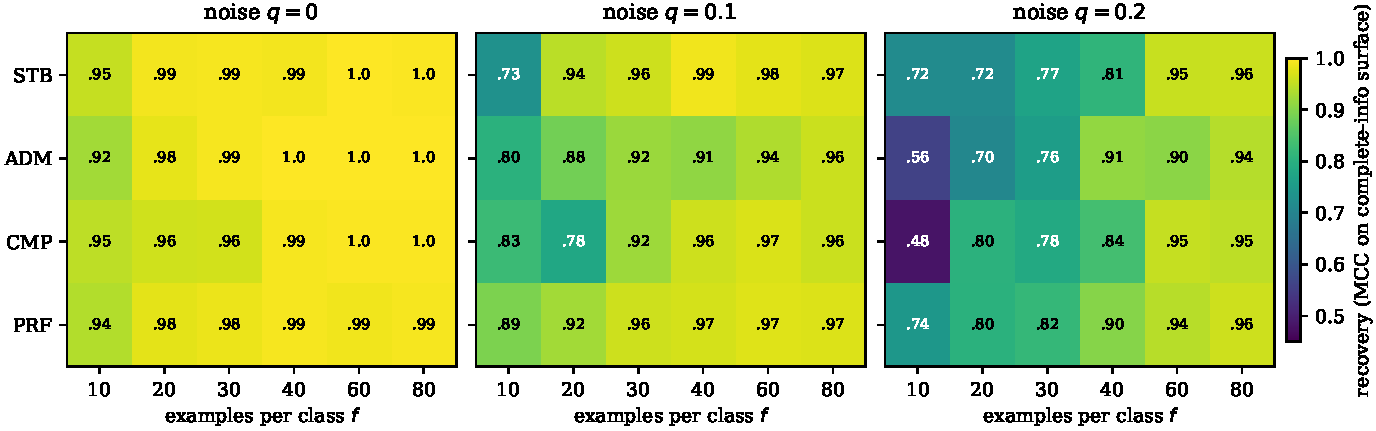
\includegraphics[width=\linewidth]{figs/fig_recovery_heatmap.pdf}
\caption{The recovery surface of Table~\ref{tab:surface} as a heatmap (brighter
$=$ better recovery). At clean labels ($q=0$) recovery is near-perfect from
$f\ge30$; noise darkens the surface, and the damage is concentrated at small
$f$ and worst for admissible/complete --- but every semantics recovers to the
bright band as $f$ grows.}
\label{fig:recovery_heatmap}
\end{figure}

\begin{figure}[t]
\centering
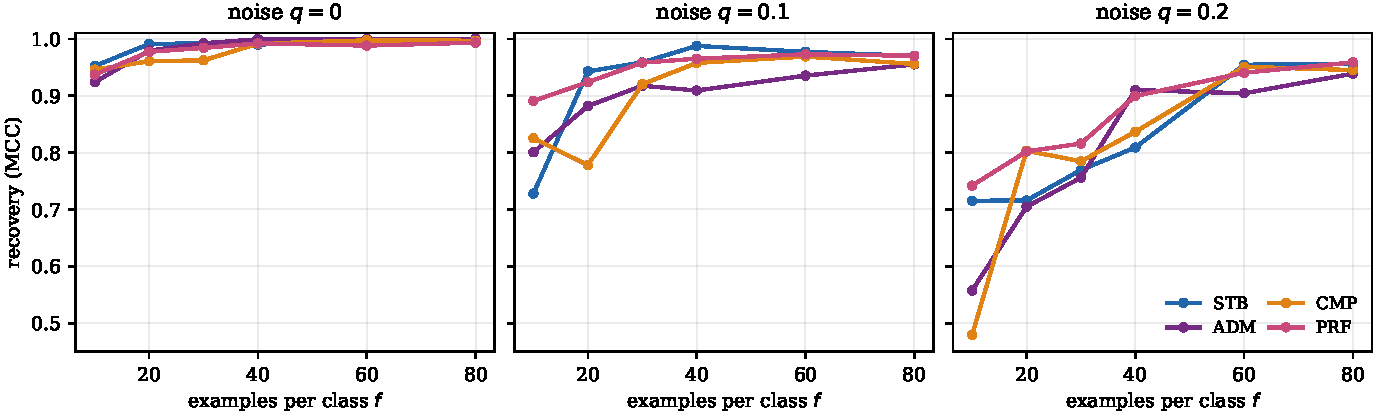
\includegraphics[width=\linewidth]{figs/fig_recovery_curves.pdf}
\caption{The same surface as recovery-vs-sample-size curves, one line per
semantics. The ``noise is bought back by data'' effect (E1.2) is the upward
slope in the $q=0.2$ panel: recovery rises from $0.48$--$0.74$ at $f=10$ to
$0.94$--$0.96$ at $f=80$, with no plateau below clean performance.}
\label{fig:recovery_curves}
\end{figure}

\begin{table}[t]
\centering
\small
\caption{The completeness--noise interaction: mean recovery by label
completeness $p$ and noise $q$ (balanced arm, pooled over semantics and $f$;
$n$ = completed runs of $120$ per cell). Incompleteness alone is free ---
recovery at $q{=}0$ is flat-to-rising as $p$ falls --- but it amplifies noise:
at $q{=}0.2$ the drop from $p{=}1.0$ to $p{=}0.5$ is $0.25$ MCC, on the
surviving runs of a cell that also loses a third of its runs to timeouts.}
\label{tab:pq}
\begin{tabular}{lccc}
\toprule
 & $q=0$ & $q=0.1$ & $q=0.2$\\
\midrule
$p=1.0$  & 0.973 \,(120) & 0.926 \,(120) & 0.872 \,(120)\\
$p=0.75$ & 0.982 \,(120) & 0.941 \,(119) & 0.864 \,(120)\\
$p=0.5$  & 0.988 \,(120) & 0.886 \,(116) & 0.619 \,(80)\\
\bottomrule
\end{tabular}
\end{table}

\begin{figure}[t]
\centering
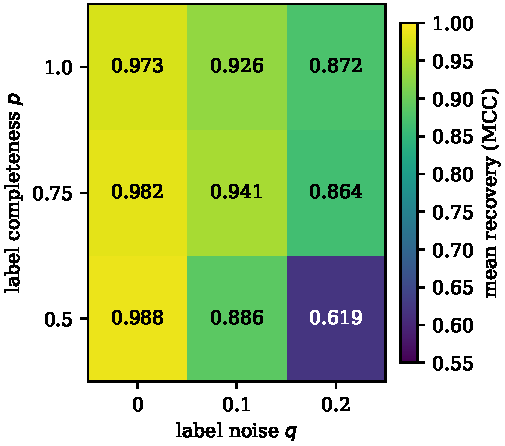
\includegraphics[width=0.5\linewidth]{figs/fig_pq_interaction.pdf}
\caption{The completeness--noise interaction (Table~\ref{tab:pq}) as a heatmap.
The top row (clean labels) is uniformly bright regardless of completeness; the
bottom-right cell (half the labels missing \emph{and} noisy) is the only dark
one --- incompleteness is free alone but multiplies the cost of noise.}
\label{fig:pq}
\end{figure}

\noindent Three headline findings.

\textbf{(E1.1) Clean-label recovery is near-perfect and fast.} At $q=0$ every
semantics exceeds MCC $0.96$ from $f\ge 30$ and is at or near $1.0$ by
$f\ge 40$; learning takes seconds (median $6$--$12$\,s per task at $q=0$). The
learned theories are typically compact \emph{constraint-style} presentations
over the guessing background rather than the definite programs of
Figure~\ref{fig:learned} --- the most frequent clean-run stable hypothesis is
\texttt{:- defeated(X), not out(X).}\ \texttt{:- supported(X), not in(X).},
which over the guessing background characterizes exactly the stable
labellings. The exact-model test scores each learned presentation on the
$100{+}100$ sampled held-out labellings, so rows below MCC $1.0$ correspond to
presentations that are only approximately extensionally correct --- the test
measures behavioural agreement on the sample, not syntactic identity or proved
equivalence.

\textbf{(E1.2) Noise is the binding constraint --- amplified by incompleteness,
bought back by data.} Label noise, not sample size or partiality, is what
degrades recovery: at $q=0.2$, small-sample recovery drops to $0.48$--$0.74$,
but every semantics climbs back to $0.94$--$0.96$ by $f=80$ (on completed
runs; see the survivorship accounting below). The completeness axis
(Table~\ref{tab:pq}) sharpens this: partial labels cost \emph{nothing} on
clean data --- if anything they help, since partial positives constrain less
and are easier to cover --- but they multiply the damage of noise
($0.872\to0.619$ at $q=0.2$ as $p$ falls from $1.0$ to $0.5$). Figures
\ref{fig:slice_noise} and~\ref{fig:slice_partial} make the interaction concrete
at a single sample size ($f=20$, where all cells are complete): under
\emph{full} labels the noise response is gentle and its fold-to-fold
variance small, whereas under \emph{half} labels the same noise both lowers
recovery and inflates its variance sharply (Figure~\ref{fig:slice_noise}); and
sweeping completeness directly (Figure~\ref{fig:slice_partial}) shows the lines
essentially flat on clean data but fanning downward once noise is present.
Recovery is \emph{not} saturated by sample size alone at imperfect information
--- the $f$-axis keeps paying off precisely when labels are partial or noisy, a
correction to the ``saturation at $f\ge 30$'' reading a clean-label study
would suggest.

\begin{figure}[t]
\centering
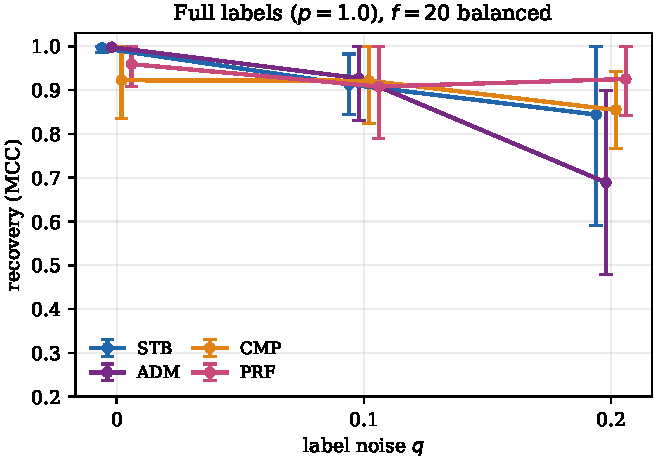
\includegraphics[width=0.49\linewidth]{figs/fig_slice_noise_full.pdf}\hfill
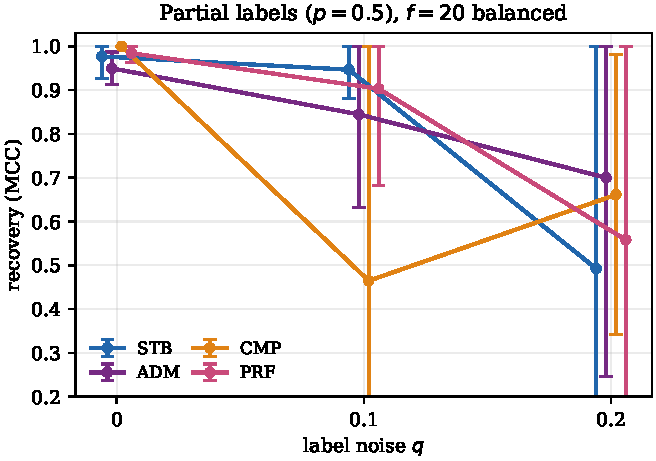
\includegraphics[width=0.49\linewidth]{figs/fig_slice_noise_partial.pdf}
\caption{Recovery versus label noise at a fixed, fully-complete sample size
($f=20$, balanced arm), with full labels ($p=1.0$, left) and half labels
($p=0.5$, right). Error bars are $95\%$ confidence intervals over the five
cross-validation folds (clipped to the valid MCC range). Partial labels turn a
gentle, low-variance noise response into a steep, high-variance one --- the same
noise is far more damaging when labels are also incomplete.}
\label{fig:slice_noise}
\end{figure}

\begin{figure}[t]
\centering
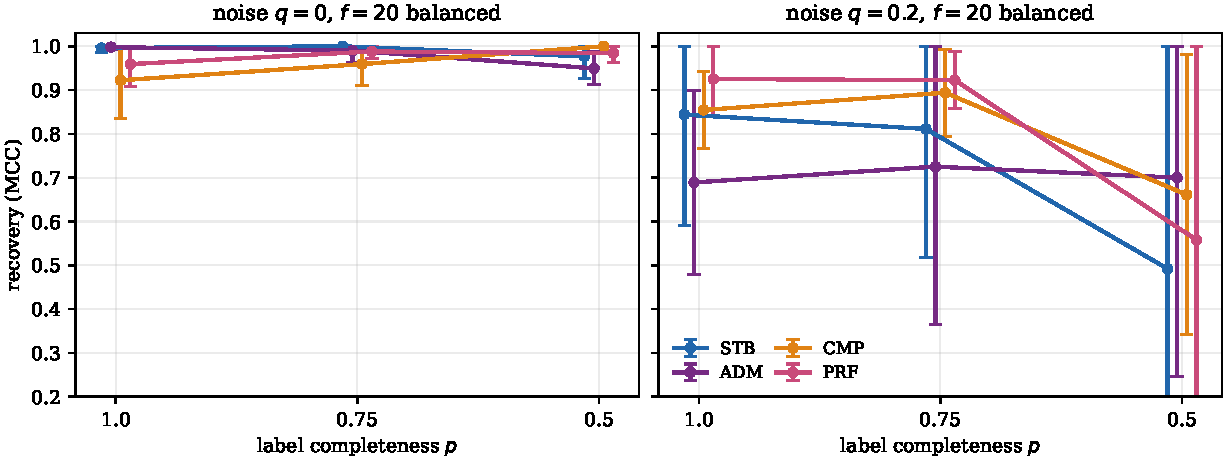
\includegraphics[width=\linewidth]{figs/fig_slice_partial.pdf}
\caption{Recovery versus label completeness at fixed $f=20$ (balanced arm), on
clean labels ($q=0$, left) and noisy labels ($q=0.2$, right); $95\%$
fold-level confidence intervals. Completeness is almost irrelevant when labels
are clean (flat lines, tight intervals) but costly and variance-inflating once
noise is present --- the interaction of Table~\ref{tab:pq} resolved per
semantics.}
\label{fig:slice_partial}
\end{figure}

\textbf{(E1.3) Class imbalance is immaterial.} Matched cell-for-cell across the
three proportion arms (Table~\ref{tab:imbalance}; $52$--$54$ matched cells per
semantics, $212$ in total), the paired contrasts are: $40\%$ vs $50\%$
$-0.009$ ($95\%$ CI $-0.021$ to $+0.003$); $60\%$ vs $50\%$ $+0.003$ ($-0.009$
to $+0.015$); $60\%$ vs $40\%$ $+0.013$ ($-0.000$ to $+0.025$). Every interval
covers or brushes zero and the largest point estimate is $0.013$ MCC ---
practically negligible even if the borderline $60$-vs-$40$ contrast were real.
The arm-mean spread decays from $0.035$ at total training size $20$ to $0.005$
at $160$ (max$-$min of the three arm means over matched cells at each total).
Balanced training sets are a convenience, not a requirement.

\begin{table}[t]
\centering
\small
\caption{Class imbalance: mean recovery per positive-fraction arm over the
cells present in all three arms (matched on semantics, completeness, noise, and
total training size; $52$--$54$ matched cells per semantics --- matching
requires at least one completed run per arm).}
\label{tab:imbalance}
\begin{tabular}{lcccc}
\toprule
Semantics & $40\%$ pos & $50\%$ pos & $60\%$ pos & max spread\\
\midrule
STB & 0.916 & 0.912 & 0.933 & 0.021\\
ADM & 0.888 & 0.889 & 0.901 & 0.013\\
CMP & 0.863 & 0.889 & 0.888 & 0.026\\
PRF & 0.912 & 0.928 & 0.908 & 0.020\\
\bottomrule
\end{tabular}
\end{table}

\begin{figure}[t]
\centering
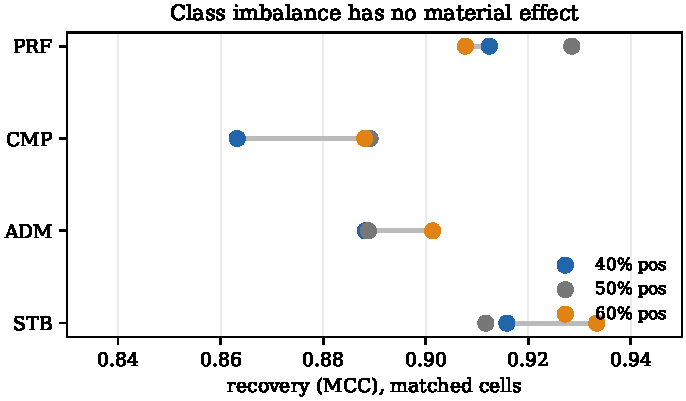
\includegraphics[width=0.62\linewidth]{figs/fig_imbalance.pdf}
\caption{Class imbalance (Table~\ref{tab:imbalance}): the $40\%$, $50\%$ and
$60\%$-positive arms sit almost on top of each other for every semantics ---
the three markers span at most $0.026$ MCC, with no consistent ordering.}
\label{fig:imbalance}
\end{figure}

\subsection{Cost and failure frontier}
\label{sec:exp1cost}

Of $3{,}240$ runs, $3{,}120$ completed, $120$ timed out at the $3{,}500$\,s
cap, and \emph{none} ended unsatisfiable or in error. The failure mass is
sharply localized: zero timeouts at $q=0$, $18$ at $q=0.1$, $102$ at $q=0.2$,
concentrated at large $f$ and low $p$ --- the same corner where median training
time rises from seconds (clean) to hundreds of seconds (noisy;
Figure~\ref{fig:time_heatmap}): learning under
noise is an optimization over exception sets, and its cost, like its accuracy
loss, is driven by the noise axis. The exclusions are material where E1.2's
high-noise recovery claim lives: on the balanced arm at $q=0.2$, $55/60$ runs
completed at $f=40$, $45/60$ at $f=60$, and $42/60$ at $f=80$. The reported
means are therefore conditional on completion; under the worst-case sensitivity
of scoring every timed-out run as MCC $0$, the $q=0.2$ pooled means would fall
from $0.937$ to $0.703$ ($f=60$) and from $0.950$ to $0.665$ ($f=80$). The
honest reading is a joint accuracy--compute claim: \emph{within the compute
budget, noise costs either accuracy or completions}; the taxonomy makes the
trade explicit instead of hiding it.

\begin{figure}[t]
\centering
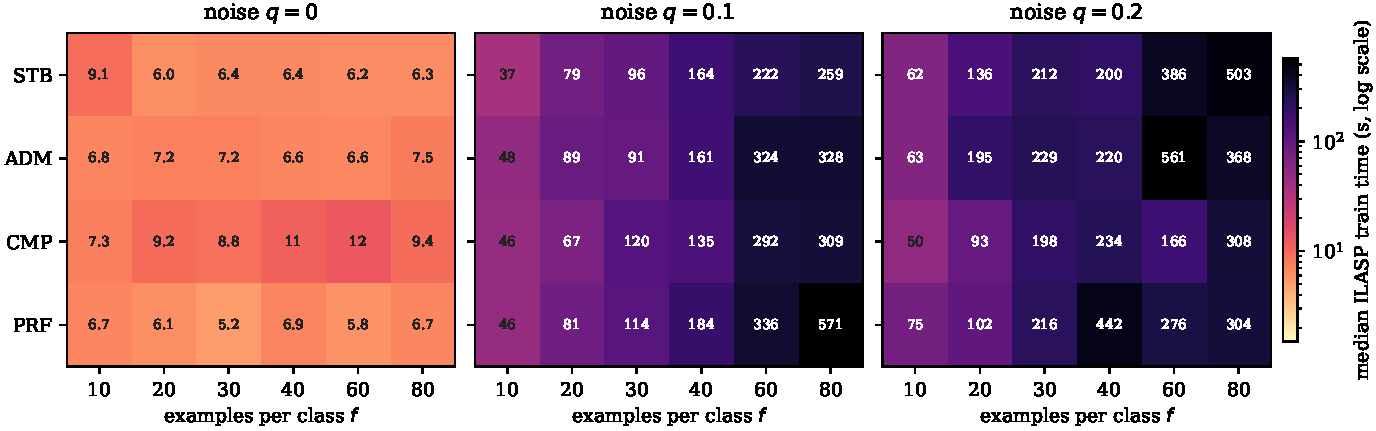
\includegraphics[width=\linewidth]{figs/fig_time_heatmap.pdf}
\caption{Median ILASP training time (log colour scale; darker $=$ slower),
same axes as Figure~\ref{fig:recovery_heatmap}. Clean cells cost seconds
(bright); adding noise darkens the surface by \emph{orders of magnitude} --- up
to $\sim$$570$\,s at the top-right --- so the cost frontier and the accuracy
frontier are driven by the same noise axis. Cells that exceeded the $3{,}500$\,s
cap are excluded from the median (Section~\ref{sec:exp1cost}).}
\label{fig:time_heatmap}
\end{figure}

\subsection{Breadth: other generators, other frameworks}
\label{sec:exp1breadth}

Three follow-up experiments test whether Experiment~1's conclusions are
artifacts of its generator regime or of the AAF setting.

\paragraph{Generator breadth.} We re-ran an anchor slice of the grid
($p\in\{1.0,0.5\}$, $q\in\{0,0.1\}$, $f\in\{20,60\}$, five folds) on three
structurally different pools: \emph{sparse} frameworks (attack count uniform in
$[n,2n]$ --- the regime of most benchmark and human-scale graphs),
\emph{self-attacking} frameworks (self-attacks permitted), and \emph{larger}
frameworks ($n\in\{10,11,12\}$). Figure~\ref{fig:generator_breadth} compares
recovery at $f=60$ against the dense pool; the finding is not a flat ``it
reproduces everywhere'' but a sharper, regime-dependent one.

\emph{Clean labels reproduce across all three regimes.} At $q=0$ every
generator recovers every semantics at MCC $\ge 0.99$ for stable, admissible,
and complete, and $\ge 0.97$ for preferred (bar one exception below) --- the
learnability of the semantics does not depend on the generator, and in
particular it \emph{scales to $n=12$}, where clean-label recovery is $0.99$--
$1.00$ throughout. This is the core robustness claim, and it holds cleanly.

\emph{Under noise the regimes separate.} Sparse tracks the dense pool closely
(within $\pm0.03$ at matched coordinates, and \emph{better} for complete, $0.94$
vs.\ $0.69$ at $f{=}20$ --- sparser graphs are if anything easier). Larger
frameworks confirm scaling but with heavier censoring: $25$ of their $160$ runs
hit the $3{,}500$\,s cap (versus $1$ for sparse), so the surviving noisy-large
numbers are survivor-biased upward and we read them as suggestive, not
definitive. The one genuine boundary is \emph{preferred on self-attacking
frameworks}: PRF recovery falls to $0.71$ at $q{=}0.1,f{=}60$ (and $0.42$ at
$f{=}20$), well below the $0.94$--$0.97$ the other regimes hold, and it is
depressed even at clean labels ($0.87$ vs.\ $0.98$). Self-attacks complicate
conflict-freeness and subset-maximality --- a self-attacking argument is in no
admissible set --- so the maximality-based construction is the most fragile
under label noise. We report this as a documented limitation of the current
formulation, not a gap: it is a specific, mechanistically explained boundary,
and the other three semantics remain robust across all three generators.

\begin{figure}[t]
\centering
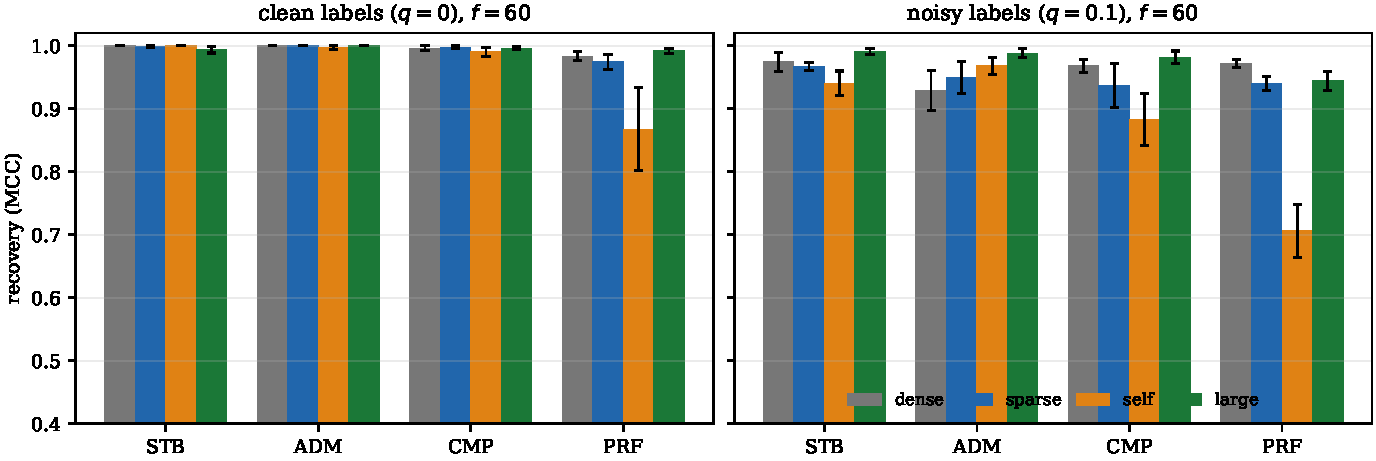
\includegraphics[width=\linewidth]{figs/fig_generator_breadth.pdf}
\caption{Generator breadth at $f=60$: recovery on the dense pool vs.\ sparse,
self-attacking, and larger ($n{\le}12$) frameworks, clean (left) and noisy
(right); bars are means over label completeness $\{1.0,0.5\}$ and five folds,
with $\pm1$ s.e.m. Clean recovery reproduces across all generators; under noise,
sparse and larger frameworks stay high (larger with heavier timeout censoring,
$25/160$), while \emph{preferred on self-attacking frameworks} is the one
regime that degrades --- a mechanistically explained boundary, not an artifact.}
\label{fig:generator_breadth}
\end{figure}

\paragraph{Framework breadth: BAF.} Using the \emph{proved} encodings of
Theorem~\ref{thm:baf} as labelling oracles, we generated 500 random BAFs
(support pairs disjoint from attacks, count uniform in $[0,n]$) and ran the
identical pipeline with background $B_{\mathrm{BAF}}$ --- and, pointedly, the
\emph{unchanged} AAF mode bias: the hypothesis space does not know supports
exist; only the background interprets them. Table~\ref{tab:breadth} (left;
Figure~\ref{fig:breadth}):
all three BAF semantics are recovered at MCC $0.85$--$0.95$ from $10$ examples
per class and $0.97$--$1.00$ from $20$, in under $9$ seconds per task (median
$4$\,s). The unifying claim of Section~\ref{sec:framework} is thus not only
verified but \emph{learnable}: one hypothesis space serves both families.

\paragraph{Framework breadth: ABA.} We generated 300 random flat ABA
frameworks, translated them with the \emph{corrected} construction of
Section~\ref{sec:abatranslation}, and ran the standard AAF pipeline on the
translated pool (which organically contains self-attacking arguments ---
assumptions attacking themselves via their own contrary).
Table~\ref{tab:breadth} (right): both tested semantics reach exact recovery
(MCC $1.0$ in every fold) by $f=40$. The end-to-end path ABA $\to$ corrected
translation $\to$ learning $\to$ verified evaluation closes the loop the
defect of Section~\ref{sec:abadefect} had broken.

\begin{table}[t]
\centering
\footnotesize
\setlength{\tabcolsep}{3pt}
\caption{Framework breadth (label completeness $1.0$, no noise, $5$ folds;
mean MCC with worst fold in parentheses). Left: BAF cells, learned with the
unchanged AAF mode bias over $B_{\mathrm{BAF}}$ ($80$ test instances per
class). Right: cells on ABA-translated AAFs via the corrected translation
($15$ test instances per class --- over half of random flat ABAs have no stable
extension, capping the per-fold test yield).}
\label{tab:breadth}
\begin{tabular}{lccc@{\quad}lccc}
\toprule
BAF & $f{=}10$ & $f{=}20$ & $f{=}40$ & ABA & $f{=}10$ & $f{=}20$ & $f{=}40$\\
\midrule
stb & 0.949 (0.89) & 0.976 (0.93) & 0.974 (0.89) & stb & 0.875 (0.62) & 0.974 (0.94) & 1.000 (1.00)\\
adm & 0.880 (0.65) & 1.000 (1.00) & 0.990 (0.95) & adm & 0.879 (0.76) & 0.974 (0.94) & 1.000 (1.00)\\
cmp & 0.848 (0.69) & 0.983 (0.94) & 0.974 (0.89) & & & &\\
\bottomrule
\end{tabular}
\end{table}

\begin{figure}[t]
\centering
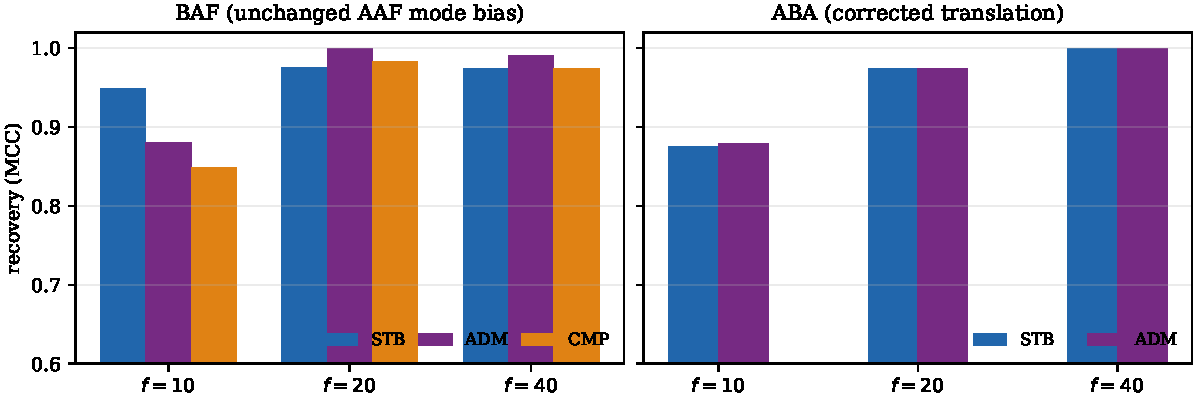
\includegraphics[width=\linewidth]{figs/fig_breadth.pdf}
\caption{Framework breadth (Table~\ref{tab:breadth}): recovery on bipolar
frameworks (learned with the \emph{unchanged} AAF hypothesis space over
$B_{\mathrm{BAF}}$) and on ABA-translated frameworks (via the corrected
translation of Section~\ref{sec:abadefect}). Both reach near-perfect recovery by
$f=20$--$40$, confirming that one learner serves all three families.}
\label{fig:breadth}
\end{figure}

%=====================================================================
\section{From Synthetic Recovery to Human Judgements: the Bridge}
\label{sec:bridge}

Experiment~1 is not only a robustness study; it is the \emph{calibration
instrument} that makes Experiment~2's conclusions safe. Four specific licenses
carry over.

\textbf{(B1) The pipeline is not the bottleneck --- and the gate proves it in
Experiment 2's own currency.} We operationalize pipeline soundness as a hard
\emph{synthetic gate}: every behavioural pipeline variant must first recover
clean \emph{textbook} labels end-to-end on the very graphs of the human study,
scored with Experiment~2's own metric, before any human-data result from it is
reported. On the grounded-semantics gate, all three pipeline variants (ILASP
at rule arity one, FastLAS OPL, FastLAS NOPL) score $1.000$ on both the
three-valued gate metric (pass threshold $0.95$) and committed-only accuracy
($n=495$). The gate also \emph{caught} a real limitation: on the
stable-semantics gate, ILASP's arity-one setting reaches only $0.921$ on the
gate metric (fail) and $0.882$ committed-only --- an expressivity ceiling of
that restricted
configuration on these graphs, which the ILASP rows of
Section~\ref{sec:exp2} therefore inherit as an explicit caveat. This is the
metric-level license: when a \emph{gated} learner trained on human labellings
falls short of a catalogue semantics, the shortfall cannot be attributed to the
learning machinery. Experiment~1's surface adds the sampled-data envelope
behind it: at behavioural sample sizes and clean labels, recovery is
$\ge0.92$ MCC (Table~\ref{tab:surface}, $q=0$).

\textbf{(B2) Oracle-free negatives are principled.} Synthetic learning enjoys
an oracle that certifies negatives; human data has none. A dedicated
calibration --- injecting per-argument label-flip noise into training positives
and comparing negative-generation policies by recovery against a clean oracle
--- found that from $f\ge 30$ examples per class, near-miss negatives generated
by flipping a single argument's label (Hamming-1 perturbation) matched
oracle-certified negatives' recovery to within fold-level variation on clean
positives; under rising injected noise, the density-based reliable-negative
policy tracked the oracle ceiling best while single-flip negatives degraded
fastest. Experiment~2 therefore pairs Hamming-1 shells with \emph{soft}
penalties --- so a wrong near-miss negative can be out-voted rather than
enforced --- and balances negative against positive penalty mass
(Section~\ref{sec:exp2setup}). \todo{re-run the calibration harness with a
persisted per-fold CSV and inline the table here; qualitative conclusions
stated per the calibration log.}

\textbf{(B3) Error decomposes --- with the interaction read the right way.}
Reading Experiment~1's surface at coordinates matching the behavioural data
yields the \emph{recovery limit}: the best any learner could do if humans
followed some Dung-style semantics exactly but reported it imperfectly. The gap
between that limit and observed human-data accuracy is then attributable to
\emph{model mismatch} --- the extent to which human acceptance is not any such
semantics. Table~\ref{tab:pq} supplies the needed calibration facts:
incompleteness alone (humans abstaining) is essentially free for the learner,
noise alone (humans erring) is survivable and data-recoverable --- but their
\emph{combination} is what collapses recovery. Since the human corpus is both
small and heterogeneous, the decomposition warns that the learner will sit at
its recovery limit long before it exhausts the signal --- anticipating the
finding that the residual gap to CF2 is individual variation rather than a
missing structural principle (Section~\ref{sec:humansem}).

\textbf{(B4) The wide search is affordable.} ILASP's expressivity makes wide
hypothesis spaces expensive on noisy behavioural tasks ($74$--$135$\,s per
call in our setting). A reformulation insight --- learn a
\emph{verifier} of a labelling given as input, rather than the labelling as a
recursive target --- makes the task representable for FastLAS, which learns the
same theories $30$--$600\times$ faster ($0.2$--$0.3$\,s), byte-identical on
clean data (Section~\ref{sec:eval}). This is what makes the enriched feature
vocabulary and the multi-seed, multi-condition protocol of Experiment~2
computationally routine.

%=====================================================================
\section{Experiment 2: Learning the Semantics Humans Use}
\label{sec:exp2}

\citet{guillaume2022} established that, among textbook semantics, \emph{CF2}
best predicts how people accept and reject arguments. The result is
\emph{descriptive}: it selects the closest member of a fixed catalogue but does
not say what acceptance principles humans apply, nor whether those principles
can be \emph{learned} from behaviour. We revisit their data with the calibrated
machinery of Sections~\ref{sec:exp1}--\ref{sec:bridge}.

\subsection{Data, protocol, audit}
\label{sec:exp2setup}

We use the accept/reject/undecided judgements of the \citet{guillaume2022}
participants across seven conditions A--G: conditions A/B/C present a
four-argument \emph{floating-reinstatement} graph, D/E/F a three-argument
acyclic graph, and G a five-argument odd cycle; conditions sharing a structure
differ in argument \emph{content}. The study recruited $130$ participants; the
individual-graph pool analysed here comprises $129$ participants' final
drawings (one condition-G participant has none), each carrying a three-valued
labelling --- the study's $495$ argument-level responses.

Each labelling enters learning as a \emph{soft} positive example, pinned by a
soft negative shell: its Hamming-1 perturbations plus one all-undecided
labelling per graph (so that totality is representable). Penalty mass is
balanced so no correct semantics can be \emph{forbidden} by an example --- only
out-voted (Section~\ref{sec:bg-las}). Prediction is generate-and-test: guess a
labelling, keep those the learned constraints admit, project credulously to a
verdict per argument.

\paragraph{Metrics.} The primary metric is \emph{committed-only accuracy}: on
responses where a human took a stance (\pred{in}/\pred{out}), the fraction the
model predicts exactly, an undecided prediction counting as wrong. A uniform
coin scores $50\%$ and a three-way guesser $33.3\%$; the empirical
majority-class baseline (predict \pred{in} everywhere) scores $0.545$ on the
committed pool ($169$ \pred{in} vs $141$ \pred{out} responses). We also report
three-valued exact match under the skeptical reading of \citet{guillaume2022}
(chance $33.3\%$). Significance: exact two-sided McNemar tests against the
pre-registered comparator CF2, deduplicated to one unit per (graph, labelling,
argument) cell --- the estimand is thus \emph{distinct response patterns}, not
participant-weighted behaviour, which removes within-cell response
multiplicity.

\paragraph{Audit.} Every reported number survives an adversarial audit:
cross-validation folds are cut at distinct (graph, labelling) cells so no
held-out response's exact training example can leak (including across
conditions D/E/F, which share graphs); all-undecided participants are retained,
reproducing the study's $495$-response pool exactly; each pipeline is gated on
clean textbook labels before any human result is trusted (B1 --- including the
disclosed ILASP stable-gate shortfall); and our textbook
baselines reproduce the published individual-graph accuracy column to within
$1.2$ points. We flag this prominently because our own first pass produced an
\emph{inflated} learner-vs-catalogue gap through three pipeline artifacts
(hard-negative contamination, choice-rule prediction inflation, and a deflated
macro-average) and an unreachable gold standard; all were found by the audit,
fixed, and the analysis re-run --- the direction of every conclusion below
survived, with honest magnitudes.

\subsection{The apples-to-apples test: learning does not beat CF2}
\label{sec:act1}

Table~\ref{tab:act1} compares, on identical held-out responses, the textbook
semantics against ILASP (at maximum rule arity one --- larger arities strictly
overfit) and FastLAS in both observational and non-observational modes.

\begin{table}[t]
\centering
\small
\caption{Experiment 2: apples-to-apples comparison on the individual-graph
pool ($n{=}495$). ``Skept.'' is three-valued exact match under the skeptical
reading (chance $33.3\%$); ``\co{}'' is committed-only accuracy under the
credulous reading. Learned theories are agnostic (no target semantics); learner
rows use the pipeline's canonical fold seed ($20260703$, fixed at run time ---
the most learner-favourable of the four seeds later used in
Table~\ref{tab:aux}, which makes the learner-below-CF2 conclusion
conservative). The ILASP row inherits the arity-one expressivity caveat flagged
by the stable gate (Section~\ref{sec:bridge}, B1). Best learner and best
overall per column in \best{bold}.}
\label{tab:act1}
\begin{tabular}{lcccc}
\toprule
& \multicolumn{2}{c}{\emph{final} (post-deliberation)} &
\multicolumn{2}{c}{\emph{first} (initial)}\\
\cmidrule(lr){2-3}\cmidrule(lr){4-5}
Predictor & Skept. & \co & Skept. & \co\\
\midrule
ILASP (arity 1)   & 0.465 & 0.410 & 0.364 & 0.206\\
FastLAS OPL       & 0.459 & \best{0.594} & 0.386 & 0.424\\
FastLAS NOPL      & 0.459 & \best{0.594} & 0.358 & 0.483\\
\midrule
grounded          & 0.562 & 0.545 & 0.483 & 0.455\\
complete          & 0.562 & 0.774 & 0.483 & 0.667\\
stable            & 0.622 & 0.742 & 0.535 & 0.648\\
preferred         & 0.638 & 0.774 & 0.539 & 0.670\\
CF2               & \best{0.648} & \best{0.797} & \best{0.556} & \best{0.692}\\
\bottomrule
\end{tabular}
\end{table}

\noindent\textbf{Every learner loses to CF2}, in both deliberation phases. The
deficit is significant under the skeptical (three-valued exact-match) reading
of the conservative cell-level McNemar test (final pool: FastLAS $27$
learner-only vs.\ $54$ CF2-only discordant cells, $p=0.004$; ILASP $14$ vs.\
$37$, $p=0.002$); under the committed-only reading the point deficit is large
($0.594$ vs $0.797$) but the deduplicated cell-level test is underpowered and
does not reach significance (FastLAS $31$ vs $35$, $p=0.71$), with the
response-level test significant for FastLAS ($49$ vs $85$, $p=0.002$). The \citeauthor{guillaume2022} conclusion is
thus robust not only to a second inference engine but to the far stronger test
of whether the semantics can be \emph{learned} from the data at all. Two
secondary findings: identical theories from FastLAS's two modes on clean
final-phase data (extra expressive power buys nothing), and a marked
learner-side degradation on noisy initial responses --- ILASP's \co{} halves
($0.410\to0.206$) and FastLAS loses $11$--$17$ points where CF2 loses $10.5$
--- learning \emph{absorbs} first-impression noise into the theory where a
fixed semantics is largely immune, the noise-sensitivity mechanism quantified
on the synthetic surface (E1.2).

\subsection{The contextual-reasoning test: one semantics, not seven}
\label{sec:act3}

Do people apply \emph{different} semantics to different graphs? Descriptively
the data flirts with this --- grounded fits condition A but collapses on B; only
CF2 commits on the odd cycle G. We test the hypothesis directly: for each
condition, compare \textsc{within} (theory trained on that condition alone),
\textsc{global} (one theory pooled over all seven), and \textsc{transfer}
(trained on the other six, identity-guarded) on identical held-out responses.
If a condition has its own semantics, \textsc{within} should beat
\textsc{global} despite less data --- a deliberately conservative reading. The
feature vocabulary here is the auxiliary one introduced in
Section~\ref{sec:aux}; the conclusions are unchanged under the primitive
vocabulary.

\begin{table}[t]
\centering
\small
\caption{Experiment 2, contextual-reasoning test (committed-only accuracy,
\emph{final} pool, auxiliary vocabulary).}
\label{tab:act3}
\begin{tabular}{llccccc}
\toprule
Cond. & Type & \#cells & \textsc{within} & \textsc{global} & \textsc{transfer} & CF2\\
\midrule
A & float  & 10 & 0.593 & 0.611 & 0.518 & \best{0.852}\\
B & float  &  6 & 0.250 & 0.900 & 0.625 & \best{1.000}\\
C & float  & 11 & 0.450 & 0.450 & \best{0.850} & 0.850\\
D & simple &  5 & \best{0.763} & 0.579 & 0.447 & 0.763\\
E & simple &  5 & 0.618 & 0.941 & 0.676 & \best{0.971}\\
F & simple &  7 & \best{0.690} & 0.552 & 0.448 & 0.690\\
G & cycle  & 19 & 0.480 & 0.560 & 0.600 & \best{0.600}\\
\bottomrule
\end{tabular}
\end{table}

The strong hypothesis is \textbf{rejected} (Table~\ref{tab:act3}): under
direction-gated, Holm-corrected McNemar tests, \emph{no} condition's own theory
significantly beats the pooled one (both vocabularies), and pooled across
conditions the effect significantly \emph{reverses}: $53$ \textsc{global}-only
vs.\ $32$ \textsc{within}-only discordant units, exact McNemar $p=0.03$.
Condition-specific theories also remain significantly below CF2 pooled ($33$
vs.\ $16$ discordant units, $p=0.02$). The pooled tests run at the
deduplicated per-argument level --- one unit per (cell, argument) pair, finer
than the (graph, labelling) cells counted in the table, which is why discordant
counts can exceed the cell column. In conditions C and G the
\textsc{transfer} theory --- trained without ever seeing the condition ---
matches CF2 and beats the condition's own theory: those participants' semantics
is not merely shared but \emph{importable}, and their noisier own-data actively
harms a specialized learner. The one within-advantage that replicates across
both vocabularies is condition D, and it is under-powered ($5$ cells). What
looks like seven semantics is one \emph{structure-sensitive} policy read
through seven structures; the context lives in the features (cycle membership,
floating reinstatement, attack load), not in per-graph switching. That policy
is the subject of the next section.

%=====================================================================
\section{The Semantics People Follow}
\label{sec:humansem}

Section~\ref{sec:act1} says the learner does not beat CF2; it does not say the
learner is uninformative. Extracting the rules that recur across
cross-validation folds (discarding per-participant noise) yields the compact,
fold-stable acceptance theory of Figure~\ref{fig:humansem} --- learned
agnostically, from behaviour alone.

\subsection{The learned theory}
\label{sec:theory}

The theory is a labelling \emph{verifier} (Section~\ref{sec:bridge}, B4): a
labelling is admissible-to-a-human unless a rule fires.

\begin{figure}[t]
\centering
\small
\fbox{\parbox{0.93\linewidth}{
\textbf{The consensus human acceptance policy} (a labelling is illegal if any
rule fires); fold stability in brackets:
\begin{description}[leftmargin=1.2em,itemsep=1.5pt,topsep=3pt]
\item[Justification] accept nothing that is not defended \hfill [5/5 folds]
\item[Commitment (acyclic)] outside cycles, a defeated argument must be
rejected and a defended one accepted --- no \pred{undec} \hfill [4/5]
\item[Cycle caution] inside a cycle, accept only the genuinely defended
\hfill [3/5]
\item[Smoke/fire] do not fully reinstate a heavily attacked argument\\
(\texttt{violated :- reinstated(X), many\_attackers(X)}) \hfill [3/5, aux.]
\end{description}}}
\caption{The human semantics $\sigma_H$ as learned. Rules 1--3 are
textbook-rational --- jointly, a \emph{committal} complete semantics with cycle
handling. Rule 4 is the psychologically distinctive hedge that no standard
Dung-style semantics encodes.}
\label{fig:humansem}
\end{figure}

Three observations locate $\sigma_H$ against the catalogue. \emph{(i)} On
acyclic graphs, rules 1--2 make $\sigma_H$ coincide with the (unique) complete
$=$ grounded $=$ preferred $=$ stable labelling \emph{with forced commitment}
--- humans do not sit on the fence when the logic is unambiguous, which is why
undecided-heavy semantics like grounded fit poorly on the simple conditions.
\emph{(ii)} On cycles, rule 3 withholds the commitment bias --- qualitatively
the direction CF2 formalizes. \emph{(iii)} Rule 4 makes $\sigma_H$
\emph{depart from every catalogue semantics}: an argument whose attackers are
all defeated is, for humans, still tainted if the attackers were many. This
violates the reinstatement principle that all Dung-style semantics
share~\citep{dung1995,baroni2011} and echoes the graded weakening of
reinstatement observed behaviourally by \citet{rahwan2010}. To our knowledge
it is the first time this hedge has been \emph{induced} from judgement data as
an explicit, checkable rule rather than posited.

We emphasize the epistemic status of $\sigma_H$: it is a fold-stable
\emph{description} of the pooled behaviour of $129$ participants on seven
graphs --- a learned consensus policy, not a proposal for a new normative
semantics; its two distinctive rules stabilize in $3$ of $5$ folds. Its value
is precisely that it is \emph{legible}: each rule can be inspected, tested on
new graphs, and traced back to the data that induced it.

\subsection{Auxiliary predicates: what closes the gap, and what does not}
\label{sec:aux}

Rule 4 references vocabulary (\pred{reinstated}, \pred{many\_attackers}) that
the primitive $\pred{arg}/\pred{att}$ language cannot state in a single
low-arity rule. We therefore searched four families of psychologically
motivated \emph{auxiliary predicates}. Two help: \emph{degree/salience}
(\pred{unattacked}, \pred{many\_attackers}, \pred{has\_unattacked\_attacker})
and \emph{reinstatement/defense} (\pred{reinstated}, \pred{floating},
\pred{undefended\_in}). Two do not --- most pointedly, \emph{SCC/cycle}
predicates, the natural vocabulary of CF2, which the learner simply ignored.
Adding the two useful families lifts committed-only accuracy from $0.571$ to
$0.648$ on average --- $+7.7$ points, positive at every one of four independent
fold seeds (range $+5.5$ to $+9.7$; an exact sign test on $n=4$ seeds gives
$p=.0625$, the minimum attainable, so the multi-seed table is offered as a
robustness check rather than an inferential claim) --- closing roughly a third
of the gap to CF2 (Table~\ref{tab:aux}).

\begin{table}[t]
\centering
\small
\caption{Auxiliary-predicate gain: committed-only accuracy (\emph{final} pool),
paired across four cross-validation seeds. Baseline $=$ FastLAS OPL, primitive
features; CF2 $= 0.797$. Seed $20260703$ (first column) is the canonical seed
used throughout Section~\ref{sec:act1}; Table~\ref{tab:act1}'s $0.594$ is that
seed's baseline value.}
\label{tab:aux}
\begin{tabular}{lccccc}
\toprule
Seed & 20260703 & 424242 & 777 & 20250101 & mean\\
\midrule
baseline & 0.594 & 0.558 & 0.558 & 0.574 & 0.571\\
$+$aux   & 0.690 & 0.642 & 0.632 & 0.629 & 0.648\\
\midrule
$\Delta$ & $+.097$ & $+.084$ & $+.074$ & $+.055$ & \best{$+.077$}\\
\bottomrule
\end{tabular}
\end{table}

The identity of the winning features is itself a finding the catalogue
comparison could not deliver: CF2's remaining edge over the learner is
\emph{not} cycle bookkeeping (else SCC predicates would help); it is a residue
of individual variation that salience and floating-reinstatement features only
partly capture. Combined with the contextual test of Section~\ref{sec:act3},
the picture is: one structure-sensitive policy, keyed on salience and
reinstatement features, with an irreducible individual-level noise floor ---
exactly the decomposition (B3) anticipated: the learner is at its recovery
limit; what remains is model mismatch between \emph{any} single semantics and a
heterogeneous population.

%=====================================================================
\section{Comparative Evaluation}
\label{sec:eval}

We close the empirical loop with the two comparisons the field most often asks
for. Both are restated from the preliminary evaluation of this
framework\footnote{arXiv:2310.12309; PAR-2 timings on a MacBook Pro M1
(2020), computing one extension per instance. The comparisons were not re-run
for this paper; we restate them with the preliminary report's own numbers,
correcting one overclaim.} rather than re-run; the correction below is ours.

\paragraph{Time performance of learned encodings.} On the ICCMA'23 benchmark
set~\citep{iccma23}, measuring PAR-2 for computing one extension: the learned
encodings are markedly faster than ASPARTIX for admissible and stable, at
parity for complete, and \emph{slower} for preferred --- where ASPARTIX's
specialized encoding outperforms our declarative subset-optimality convention.
We state this honestly, correcting the preliminary report's abstract-level
claim of outperforming existing solvers: learned encodings are competitive,
sometimes better, not uniformly dominant.

\paragraph{Data efficiency versus deep learning.} The approximate solver
AGNN~\citep{craandijkbex2020} reaches MCC $0.998$--$0.999$ for stable,
preferred, and complete after training on $10^{6}$ labelled frameworks. As
reported in the preliminary evaluation, the LAS route reaches MCC $=1.0$ ---
with a \emph{verified} theory --- from $7$ (admissible), $8$ (stable,
complete), and $16$ (preferred) examples on frameworks of at most five
arguments; conversely, capping AGNN's training set at $30$ examples collapses
it to MCC $\le 0.31$ on the semantics studied here (stable $0.054$, complete
$0.213$, preferred $0.303$). The comparison is not adversarial --- AGNN
targets amortized inference speed, not data efficiency --- but it quantifies
the regime where interpretable learning is the only viable option: when
labelled data is scarce, as in behavioural settings (Section~\ref{sec:exp2})
where the \emph{entire corpus} is $495$ responses.

\paragraph{ILP engines.} Within the LAS family: ILASP's full expressivity is
required for learning \emph{generative} encodings (choice-rule hypothesis
spaces, Section~\ref{sec:exp1}); FastLAS, under the verifier reformulation
(B4), learns constraint-style theories $30$--$600\times$ faster and identically
on clean data --- the workhorse of Experiment~2's wide-vocabulary protocol.
The reformulation is a transferable lesson: FastLAS's observational predicate
learning cannot use body features defined recursively from the learning
target; making the labelling an \emph{input} and learning its \emph{verifier}
removes the recursion without changing the semantics of the task.

\paragraph{Compactness.} The learned encodings are small: two to three rules
per semantics plus the shared background, against reference encodings of up to
$33$ rules (preferred). Every learned theory in this paper fits --- and is
displayed --- on a fraction of a page.

%=====================================================================
\section{Related Work}
\label{sec:related}

\paragraph{Computing semantics.} Reduction-based solvers, notably the ASPARTIX
family~\citep{egly2010}, encode each semantics as an ASP program; the ICCMA
competitions~\citep{iccma23} track the state of the art. We invert the
direction: encodings are induced from examples and then \emph{proved}
equivalent to the references.

\paragraph{Learning and argumentation.} Approximate acceptability solvers
learn to \emph{predict} acceptance --- AGNN~\citep{craandijkbex2020}, graph
convolutional approaches~\citep{kuhlmann2019} --- but yield black-box
predictors tied to a fixed known semantics. Closer to us, a recent ILP line
learns ABA \emph{frameworks} (rules, assumptions, contraries) from examples
--- a different inverse problem: structure given a semantics, where we learn
the semantics given structures \todo{cite Proietti \& Toni's ABA-learning line
after the literature sweep}. Our contribution is learning the \emph{semantics}
as an explicit logic program, with certified correctness. \todo{2023--2026
refresh: NeSy argumentation, newer GNN solvers, ILP for argumentation
strategies --- required before the ``first'' claims of C2 and
Section~\ref{sec:theory} are submitted.}

\paragraph{ILP / LAS.} We build directly on ILASP's context-dependent,
noise-tolerant learning~\citep{law2016,law2018,law2019,law2018phd} and
FastLAS~\citep{law2020}. The verifier reformulation (B4) relates to
observational predicate learning limits discussed by \citet{law2020}.

\paragraph{Verification of ASP.} Our completion-based level follows the
classical Clark/Fages line~\citep{clark1978,fages1994}; the external-equivalence
level uses \textsc{anthem}~\citep{anthem2020,anthem2023} with
\textsc{Vampire}~\citep{vampire}. Applying this toolchain to \emph{learned}
programs --- and using it to falsify and repair a published encoding --- is, to
our knowledge, new.

\paragraph{Human argumentation.} Behavioural studies of abstract argumentation
begin with reinstatement~\citep{rahwan2010} and culminate in the
catalogue-comparison methodology of \citet{cramer2018,guillaume2022}, which our
Experiment~2 re-analyzes. Our contribution is methodological (a leakage-free,
gated, calibrated ILP protocol with directional statistics) and substantive
(the learned policy $\sigma_H$, the feature-not-policy resolution of
contextuality, and the negative result on SCC vocabulary).

%=====================================================================
\section{Conclusions and Future Work}
\label{sec:concl}

We asked whether argumentation semantics can be learned (Q1), trusted (Q2),
learned robustly (Q3), and used as an instrument on human data (Q4). The
answers: \emph{yes} --- one background and hypothesis space covers AAF and BAF
with learning experiments and theorems, ABA via a corrected translation, and
VAF at the level of the unified background; \emph{provably} --- with
machine-checked equivalence at up to three independent levels, strong enough to
uncover and repair a published defect; \emph{yes, within a mapped envelope} ---
near-perfect recovery from clean data at $30$--$40$ examples per class, noise
as the binding but data-recoverable constraint (amplified by label
incompleteness), imbalance immaterial, clean-label recovery reproduced across
sparse, self-attacking, and larger ($n{\le}12$) generators and two further
framework families, with self-attacking preferred the one identified boundary;
and \emph{yes} --- on
human data the calibrated learner both confirms the CF2 ceiling under a
stronger-than-before test and returns what the catalogue cannot: a legible
human acceptance policy with a non-Dungian distrust of heavily attacked
arguments, and a principled rejection of per-graph semantics.

\paragraph{Limitations.} The synthetic envelope is mapped on random digraphs of
moderate size ($n\le12$). Clean-label recovery reproduces across the sparse,
self-attacking, and larger generators; under noise, larger frameworks carry
heavier timeout censoring ($25/160$ runs hit the cap, so their noisy recovery is
read as suggestive), and \emph{preferred on self-attacking frameworks} degrades
(PRF $0.42$--$0.71$ under noise) because self-attacks break the conflict-freeness
and subset-maximality the construction leans on --- a specific, mechanistically
understood boundary rather than a general failure. Grounded semantics was
scoped out of the learnability study for a diagnosed reason --- on dense pools
its extension is empty $69\%$ of the time, starving the learner's positive
signal --- and learning it under a signal-bearing sparse distribution is an
open, now well-posed problem. VAF is covered by the unified background and its
randomized specialization checks, but carries no learning experiments or
theorems of its own here. $\sigma_H$ describes pooled behaviour on seven
graphs; its two distinctive rules stabilize in $3$ of $5$ folds, its auxiliary
vocabulary was selected on the same corpus and awaits pre-registered
replication, and the contextual-reasoning test is well-powered only for the
cyclic condition G (the per-condition nulls elsewhere rest on $5$--$11$
held-out cells each). Committed-only accuracy peaks in the mid-$60$s against a
CF2 ceiling near $80\%$: closing that residue likely requires per-participant
modelling, not better features.

\paragraph{Future work.} Three directions follow directly. \emph{Custom
semantics at scale}: the machinery is agnostic to the target; learning
domain-specific acceptance policies (legal, medical, deliberative) from expert
labellings is now an engineering exercise with a calibration methodology
attached. \emph{Verified learning as a loop}: the anthem-based certification
step can run \emph{inside} learning, rejecting hypotheses not equivalent to any
admissible target --- a learn-verify loop for logic programs; the same
reduction technique should also mechanize the unified-background specialization
(C1) and the VAF case. \emph{Dialogue}: combining the learned human policy
$\sigma_H$ with argument-mining front ends to predict, and intervene on, real
deliberation.

%=====================================================================
\appendix

\section{Manual proof for the admissible case}
\label{app:proofs}
\todo{port the reduct-based proof of Theorem~\ref{thm:aaf} (admissible case)
from the precursor report; state the two errata found during mechanization.}

\section{Verification artifacts}
\label{app:artifacts}
All verification inputs and scripts ship with the repository:
\texttt{analysis/zlatina\_theorems/} (exhaustive checkers, Z3 completion
proofs, \textsc{anthem} inputs and program pairs, with per-theorem prover
logs), and the ABA defect lab (minimal counterexample and validated fix).
Prover versions: \textsc{anthem}~2 (built from source), \textsc{Vampire}~5.0.1,
Z3~4.16, clingo~5.x.

\section{Campaign details}
\label{app:campaign}
Full per-cell tables (including per-completeness surfaces beyond
Table~\ref{tab:pq}), configuration files with pinned seeds, the
failure-taxonomy ledger, and the exact generator/labeller/learner invocations
for Experiment~1 and the breadth experiments. \todo{inline the per-cell tables
and the completed breadth regimes.}

%=====================================================================
\begin{thebibliography}{99}

\bibitem[Baroni et al.(2005)]{baroni2005}
P.~Baroni, M.~Giacomin, G.~Guida.
SCC-recursiveness: a general schema for argumentation semantics.
\emph{Artificial Intelligence} 168(1--2):162--210, 2005.

\bibitem[Baroni et al.(2011)]{baroni2011}
P.~Baroni, M.~Caminada, M.~Giacomin.
An introduction to argumentation semantics.
\emph{Knowledge Engineering Review} 26(4):365--410, 2011.

\bibitem[Bench-Capon(2003)]{benchcapon2003}
T.~J.~M. Bench-Capon.
Persuasion in practical argument using value-based argumentation frameworks.
\emph{Journal of Logic and Computation} 13(3):429--448, 2003.

\bibitem[Bondarenko et al.(1997)]{bondarenko1997}
A.~Bondarenko, P.~M. Dung, R.~A. Kowalski, F.~Toni.
An abstract, argumentation-theoretic approach to default reasoning.
\emph{Artificial Intelligence} 93(1--2):63--101, 1997.

\bibitem[Caminada(2006)]{caminada2006}
M.~Caminada.
On the issue of reinstatement in argumentation.
In \emph{Proc.\ JELIA}, 111--123, 2006.

\bibitem[Cayrol and Lagasquie-Schiex(2009)]{cayrol2009}
C.~Cayrol, M.-C. Lagasquie-Schiex.
Bipolar abstract argumentation systems.
In G.~Simari, I.~Rahwan (eds.), \emph{Argumentation in Artificial
Intelligence}, 65--84. Springer, 2009.

\bibitem[Clark(1978)]{clark1978}
K.~L. Clark.
Negation as failure.
In \emph{Logic and Data Bases}, 293--322. Plenum Press, 1978.

\bibitem[Craandijk and Bex(2020)]{craandijkbex2020}
D.~Craandijk, F.~Bex.
Deep learning for abstract argumentation semantics.
In \emph{Proc.\ IJCAI}, 1667--1673, 2020.

\bibitem[Cramer and Guillaume(2018)]{cramer2018}
M.~Cramer, M.~Guillaume.
Empirical cognitive study on abstract argumentation semantics.
In \emph{Proc.\ COMMA}, 413--424, 2018.

\bibitem[de Moura and Bj{\o}rner(2008)]{z3}
L.~de Moura, N.~Bj{\o}rner.
Z3: an efficient SMT solver.
In \emph{Proc.\ TACAS}, 337--340, 2008.

\bibitem[Dung(1995)]{dung1995}
P.~M. Dung.
On the acceptability of arguments and its fundamental role in nonmonotonic
reasoning, logic programming and $n$-person games.
\emph{Artificial Intelligence} 77(2):321--357, 1995.

\bibitem[Egly et al.(2010)]{egly2010}
U.~Egly, S.~A. Gaggl, S.~Woltran.
Answer-set programming encodings for argumentation frameworks.
\emph{Argument \& Computation} 1(2):147--177, 2010.

\bibitem[Fages(1994)]{fages1994}
F.~Fages.
Consistency of Clark's completion and existence of stable models.
\emph{Journal of Methods of Logic in Computer Science} 1:51--60, 1994.

\bibitem[Fandinno et al.(2020)]{anthem2020}
J.~Fandinno, V.~Lifschitz, P.~L{\"u}hne, T.~Schaub.
Verifying tight logic programs with \textsc{anthem} and \textsc{Vampire}.
\emph{Theory and Practice of Logic Programming} 20(5):735--750, 2020.

\bibitem[Fandinno et al.(2023)]{anthem2023}
J.~Fandinno, Z.~Hansen, Y.~Lierler, V.~Lifschitz, N.~Temple.
External behavior of a logic program and verification of refactoring.
\emph{Theory and Practice of Logic Programming} 23(4):933--947, 2023.

\bibitem[Gebser et al.(2019)]{gebser2019}
M.~Gebser, R.~Kaminski, B.~Kaufmann, T.~Schaub.
Multi-shot ASP solving with clingo.
\emph{Theory and Practice of Logic Programming} 19(1):27--82, 2019.

\bibitem[Gelfond and Kahl(2014)]{gelfondkahl2014}
M.~Gelfond, Y.~Kahl.
\emph{Knowledge Representation, Reasoning, and the Design of Intelligent
Agents}. Cambridge University Press, 2014.

\bibitem[Guillaume et al.(2022)]{guillaume2022}
M.~Guillaume, M.~Cramer, L.~van~der Torre, C.~Schiltz.
Reasoning on conflicting information: an empirical study of formal
argumentation.
\emph{PLOS ONE} 17(8):e0273225, 2022.

\bibitem[J{\"a}rvisalo et al.(2023)]{iccma23}
M.~J{\"a}rvisalo, T.~Lehtonen, A.~Niskanen.
ICCMA 2023: benchmarks and raw results. Zenodo, 2023.

\bibitem[Kov{\'a}cs and Voronkov(2013)]{vampire}
L.~Kov{\'a}cs, A.~Voronkov.
First-order theorem proving and \textsc{Vampire}.
In \emph{Proc.\ CAV}, 1--35, 2013.

\bibitem[Kuhlmann and Thimm(2019)]{kuhlmann2019}
I.~Kuhlmann, M.~Thimm.
Using graph convolutional networks for approximate reasoning with abstract
argumentation frameworks: a feasibility study.
In \emph{Proc.\ SUM}, 24--37, 2019.

\bibitem[Law(2018)]{law2018phd}
M.~Law.
\emph{Inductive Learning of Answer Set Programs}.
PhD thesis, Imperial College London, 2018.

\bibitem[Law et al.(2016)]{law2016}
M.~Law, A.~Russo, K.~Broda.
Iterative learning of answer set programs from context dependent examples.
\emph{Theory and Practice of Logic Programming} 16(5--6):834--848, 2016.

\bibitem[Law et al.(2018)]{law2018}
M.~Law, A.~Russo, K.~Broda.
Inductive learning of answer set programs from noisy examples.
\emph{Advances in Cognitive Systems}, 2018.

\bibitem[Law et al.(2019)]{law2019}
M.~Law, A.~Russo, K.~Broda.
Logic-based learning of answer set programs.
In \emph{Reasoning Web: Explainable AI}, 196--231. Springer, 2019.

\bibitem[Law et al.(2020)]{law2020}
M.~Law, A.~Russo, E.~Bertino, K.~Broda, J.~Lobo.
FastLAS: scalable inductive logic programming incorporating domain-specific
optimisation criteria.
In \emph{Proc.\ AAAI}, 2877--2885, 2020.

\bibitem[Rahwan et al.(2010)]{rahwan2010}
I.~Rahwan, M.~I. Madakkatel, J.-F. Bonnefon, R.~N. Awan, S.~Abdallah.
Behavioral experiments for assessing the abstract argumentation semantics of
reinstatement.
\emph{Cognitive Science} 34(8):1483--1502, 2010.

\end{thebibliography}

\end{document}
